%% LyX 2.5.1 created this file.  For more info, see https://www.lyx.org/.
%% Do not edit unless you really know what you are doing.
\documentclass[journal,article,submit,moreauthors]{Definitions/mdpi}
\usepackage{textcomp}
\usepackage[utf8]{inputenc}
\synctex=-1
\usepackage{array}
\usepackage{float}
\usepackage{url}
\usepackage{multirow}
\usepackage{varwidth}
\usepackage{amsmath}
\usepackage{graphicx}

\makeatletter

%%%%%%%%%%%%%%%%%%%%%%%%%%%%%% LyX specific LaTeX commands.

\Title{The Effects of Climate Change (normal values/anomalous values) on
Fire Duration, in Greece Areas.}

\Author{Constantina Kopitsa$^{1}$, \textsubscript{\textsuperscript{}}Ioannis
G. Tsoulos$^{2*}$, Vasileios Charilogis$^{3}$}


\address{$^{1}\quad$Department of Informatics and Telecommunications. University
of Ioannina, \\
$^{2}\quad$Department of Informatics and Telecommunications. University
of Ioannina, \\
$^{3}\quad$Department of Informatics and Telecommunications. University
of Ioannina, }


\corres{Correspondence: itsoulos@uoi.gr}


\abstract{In this study, we examine and highlight the effects of climate change
on forest fires duration that have afflicted Greece over the past
25 years (2000- 2025). Thus, we selected three distinct regions,of
Greece, spanning a distance of approximately 1.000 kilometers, in
order to ensure impartial findings that are not confined to a single
area and, consequently to avoid creating a misleading impression.
The first area of interest is Attica, with 2.100 rows of climatological
data and fire duration records. The second area lies further south
and is Crete, with 2.893 rows of climatological data and fire duration
records. The third area of interest is located further north and is
Eastern Macedonia \& Thrace, with 2.919 rows of climatological data
and fire duration records. The baseline for our analysis was established
using climatological data from 1980--2010 for the regions of Attica
and Crete, and from 1992--2022 for Eastern Macedonia and Thrace,
reflecting the earliest available records for that area. These datasets
were processed to derive monthly mean values representing the climatological
normal's. We then compared these normal's with the meteorological
conditions present at the onset of wildfire events during the period
2000--2025. Our findings report the climatological anomalous (climate
change) influence of: temperature, wind speed, and humidity on wildfire
duration. The machine learning techniques successfully validated our
results, with the FC2 method based on Grammatical Evolution for constructing
new features, achieving the best overall performance with mean relative
error across all three regions at 1.51\%. Specifically, the error
rate for the Attica region was 1.90\% (98.10\% accuracy), for Crete
2.18\% (97.82\% accuracy), and for the Eastern Macedonia \& Thrace
region 0.46\% (99.54\% accuracy). }


\keyword{Climate change; machine learning; neural networks}

\DeclareTextSymbolDefault{\textquotedbl}{T1}
%% Because html converters don't know tabularnewline
\providecommand{\tabularnewline}{\\}
%% Variable width box for table cells
\newenvironment{cellvarwidth}[1][t]
    {\begin{varwidth}[#1]{\linewidth}}
    {\@finalstrut\@arstrutbox\end{varwidth}}

%%%%%%%%%%%%%%%%%%%%%%%%%%%%%% User specified LaTeX commands.
%  LaTeX support: latex@mdpi.com
%  For support, please attach all files needed for compiling as well as the log file, and specify your operating system, LaTeX version, and LaTeX editor.
%=================================================================
%\documentclass[preprints,article,submit,moreauthors]{Definitions/mdpi}
% For posting an early version of this manuscript as a preprint, you may use "preprints" as the journal. Changing "submit" to "accept" before posting will remove line numbers.
% Below journals will use APA reference format:
% admsci, aieduc, behavsci, businesses, econometrics, economies, education, ejihpe, famsci, games, humans, ijcs, ijfs, investment, fclam, jintelligence, journalmedia, jrfm, jsam, languages, opermanag, peacestud, pmh, psycholint, publications, tourismhosp, youth
% Below journals will use Chicago reference format:
% arts, genealogy, histories, humanities, laws, literature, religions, risks, socsci
%--------------------
% Class Options:
%--------------------
%----------
% journal
%----------
% Choose between the following MDPI journals:
% accountaudit, acn, acoustics, actuators, addictions, addictprev, adhesives, adolescents, aerobiology, aerospace, agriculture, agriengineering, agrochemicals, agronomy, ai, aichem, aieng, aimater, aimed, aipa, air, aisens, aisoc, algorithms, allergies, alloys, amh, analog, analytica, analytics, anatomia, anesthres, animals, antibiotics, antibodies, antioxidants, applbiosci, appliedchem, appliedmath, appliedphys, applmech, applmicrobiol, applnano, applsci, aps, aquacj, archaeolstud, architecture, arm, arthropoda, asc, asi, astronautics, astronomy, atmosphere, atoms, audiolres, automation, axioms, bacteria, batteries, bdcc, beverages, biochem, bioengineering, biologics, biology, biomass, biomechanics, biomed, biomedicines, biomedinformatics, biomimetics, biomolecules, biophysica, bioresourbioprod, biosensors, biosphere, biotech, birds, blockchains, bloods, blsf, brainsci, breath, buildings, cancers, carbon, cardio, cardiogenetics, cardiovascmed, catalysts, cells, ceramics, challenges, chemengineering, chemistry, chemosensors, chemproc, children, chips, cimb, civileng, cleantechnol, climate, clinbioenerg, clinpract, clockssleep, cmd, cmtr, coasts, coatings, colloids, colorants, commodities, complexities, complications, compounds, computation, computers, condensedmatter, conservation, constrmater, cosmetics, covid, crops, cryo, cryptography, crystals, csmf, ctn, culture, curroncol, cyber, dairy, data, ddc, dentistry, dermato, dermatopathology, designs, devices, dhi, diabetology, diagnostics, dietetics, digital, disabilities, diseases, diversity, dna, drones, drugreact, drylands, dynamics, earth, ebj, ecm, ecologies, edm, eesp, electricity, electrochem, electronicmat, electronics, embodiedintell, encyclopedia, endocrines, energies, eng, engproc, entomology, entropy, environments, environremediat, epidemiologia, epigenomes, esa, est, fermentation, fibers, fintech, fire, fishes, fluids, foodeng, foods, forecasting, forensicsci, forests, fossstud, foundations, fractalfract, freshwater, fuels, future, futureinternet, futurepharmacol, futurephys, futuretransp, galaxies, gases, gastroent, gastrointestdisord, gastronomy, gels, genes, geochem, geographies, geohazards, geomatics, geometry, geosciences, geotechnics, geriatrics, germs, glacies, grainsci, grasses, green, greenhealth, gucdd, gynecolcancer, hardware, hazardousmatters, healthcare, healthcmater, hearts, hemato, hematolrep, hep, heritage, higheredu, highthroughput, horticulturae, hospitals, hydrobiology, hydrogen, hydrology, hydrometeorology, hydropower, hygiene, idr, iic, ijem, ijerph, ijgi, ijmd, ijms, ijns, ijom, ijp, ijpb, ijt, ijtm, ijtpp, ijtst, ime, immuno, industries, inflammj, informatics, information, infrastructures, inorganics, insects, instruments, inventions, iot, j, jaestheticmed, jal, japma, jcdd, jcm, jcp, jcrm, jcs, jcto, jdad, jdb, jdream, jemr, jeta, jfb, jfmk, jfth, jgbg, jgg, jimaging, jlpea, jmahp, jmmp, jmms, jmp, jmse, jne, jnt, jof, joi, joitmc, joma, jop, joptm, jor, jox, jpbi, jphytomed, jpm, jsan, jtaer, jvd, jzbg, kidneydial, kinasesphosphatases, knowledge, labmed, laboratories, lam, land, lasers, legumes, life, lights, limnolrev, lipidology, liquids, livers, logics, logistics, lubricants, lymphatics, machines, macromol, magnetism, magnetochemistry, make, marinedrugs, maritime, materials, materproc, mathematics, mca, mcb, measurements, medicina, medicines, medsci, membranes, merits, metabolites, metals, meteorology, methane, metrics, metrology, micro, microarrays, microbiolres, microelectronics, micromachines, microorganisms, microplastics, microwave, minerals, mining, mmphys, modelling, molbank, molecules, mollusca, mps, msf, mti, multimedia, muscles, nanoenergyadv, nanomanufacturing, nanomaterials, ncrna, ndt, network, neuroglia, neuroimaging, neurolint, neurosci, nitrogen, notspecified, nursrep, nutraceuticals, nutrients, obesities, occuphealth, oceans, ohbm, onco, optics, oral, organics, organoids, osteology, oxygen, pandemics, parasites, parasitologia, particles, pathogens, pathophysiology, pediatrrep, pets, pharmaceuticals, pharmaceutics, pharmacoepidemiology, pharmacy, phc, philosophies, photochem, photonics, photovoltaics, phycology, physchem, physics, physiologia, plants, plasma, platforms, pollutants, polymers, polysaccharides, populations, poultry, powders, precision, precisoncol, preprints, proceedings, processes, prosthesis, proteomes, psf, psychiatryint, psychoactives, purification, quantumrep, quaternary, qubs, radiation, rareearths, rdt, reactions, realestate, receptors, recycling, regeneration, remotesensing, reports, reprodmed, resources, rheumato, rjpm, robotics, rsee, ruminants, safety, sanpp, sca, sci, scipharm, sclerosis, seeds, sensors, separations, sexes, shi, signals, sinusitis, siuj, skins, smartcities, smartfish, sna, societies, software, soilsystems, solar, solids, spectroscj, sports, standards, stats, std, stratsediment, stresses, strokerep, superintelligence, surfaces, surgeries, suschem, sustainability, sustainfoods, sustainpackag, symmetry, synbio, systems, tae, targets, taxonomy, technologies, telecom, test, textiles, thalassrep, therapeutics, thermo, timespace, tomography, toxics, toxins, tph, transplantology, transportation, traumacare, traumas, tri, tropicalmed, universe, urbansci, uro, vaccines, vehicles, venereology, vetsci, vibration, virtualworlds, viruses, vision, waste, water, welding, wem, wevj, wild, wind, women, world, zoonoticdis
%---------
% article
%---------
% The default type of manuscript is "article", but can be replaced by:
% abstract, addendum, article, book, bookreview, briefreport, casereport, comment, commentary, communication, conferenceproceedings, correction, conferencereport, entry, expressionofconcern, extendedabstract, datadescriptor, editorial, essay, erratum, hypothesis, interestingimage, obituary, opinion, projectreport, reply, retraction, review, perspective, protocol, shortnote, studyprotocol, systematicreview, supfile, technicalnote, viewpoint, guidelines, registeredreport, tutorial
% supfile = supplementary materials
%----------
% submit
%----------
% The class option "submit" will be changed to "accept" by the Editorial Office when the paper is accepted. This will only make changes to the frontpage (e.g., the logo of the journal will get visible), the headings, and the copyright information. Also, line numbering will be removed. Journal info and pagination for accepted papers will also be assigned by the Editorial Office.
%------------------
% moreauthors
%------------------
% If there is only one author the class option oneauthor should be used. Otherwise use the class option moreauthors.
%=================================================================
% MDPI internal commands - do not modify
\firstpage{1}
\setcounter{page}{\@firstpage}
\pubvolume{1}
\issuenum{1}
\articlenumber{0}
\pubyear{2026}
\copyrightyear{2026}
%\externaleditor{Firstname Lastname} % More than 1 editor, please add `` and '' before the last editor name
\datereceived{}
\daterevised{ } % Comment out if no revised date
\dateaccepted{}
\datepublished{}
%\datecorrected{} % For corrected papers include a "Corrected: XXX" date in the original paper.
%\dateretracted{} % For retracted papers include a "RETRACTED: XXX" date in the original paper.
%\doinum{} % Used for some special journals, like molbank
%\pdfoutput=1 % Uncommented for upload to arXiv.org
%\CorrStatement{yes}  % For updates
%\longauthorlist{yes} % For many authors that exceed the left citation part
%\IsAssociation{yes} % For association journals
%=================================================================
% Add packages and commands here. The following packages are loaded in our class file: fontenc, inputenc, calc, indentfirst, fancyhdr, graphicx, epstopdf, lastpage, ifthen, lineno, float, amsmath, setspace, enumitem, mathpazo, booktabs, titlesec, etoolbox, tabto, xcolor, soul, multirow, microtype, tikz, totcount, changepage, attrib, upgreek, cleveref, amsthm, hyphenat, natbib, hyperref, footmisc, url, geometry, newfloat, caption
%=================================================================
%% Please use the following mathematics environments: Theorem, Lemma, Corollary, Proposition, Characterization, Property, Problem, Example, ExamplesandDefinitions, Hypothesis, Remark, Definition, Notation, Assumption
%% For proofs, please use the proof environment (the amsthm package is loaded by the MDPI class).
%=================================================================
% The fields PACS, MSC, and JEL may be left empty or commented out if not applicable
%\PACS{J0101}
%\MSC{}
%\JEL{}
%%%%%%%%%%%%%%%%%%%%%%%%%%%%%%%%%%%%%%%%%%
% Only for the journal Diversity
%\LSID{\url{http://}}
%%%%%%%%%%%%%%%%%%%%%%%%%%%%%%%%%%%%%%%%%%
% Only for the journal Applied Sciences:
%\featuredapplication{Authors are encouraged to provide a concise description of the specific application or a potential application of the work. This section is not mandatory.}
%%%%%%%%%%%%%%%%%%%%%%%%%%%%%%%%%%%%%%%%%%
%%%%%%%%%%%%%%%%%%%%%%%%%%%%%%%%%%%%%%%%%%
% Only for the journal Data:
%\dataset{DOI number or link to the deposited data set in cases where the data set is published or set to be published separately. If the data set is submitted and will be published as a supplement to this paper in the journal Data, this field will be filled by the editors of the journal. In this case, please make sure to submit the data set as a supplement when entering your manuscript into our manuscript editorial system.}
%\datasetlicense{license under which the data set is made available (CC0, CC-BY, CC-BY-SA, CC-BY-NC, etc.)}
%%%%%%%%%%%%%%%%%%%%%%%%%%%%%%%%%%%%%%%%%%
% Only for the journal BioTech, Fishes, Neuroimaging and Toxins
%\keycontribution{The breakthroughs or highlights of the manuscript. Authors can write one or two sentences to describe the most important part of the paper.}
%%%%%%%%%%%%%%%%%%%%%%%%%%%%%%%%%%%%%%%%%%
% Only for the journal Encyclopedia
%\encyclopediadef{Instead of the abstract}
%\entrylink{The Link to this entry published on the encyclopedia platform.}
%%%%%%%%%%%%%%%%%%%%%%%%%%%%%%%%%%%%%%%%%%
%%%%%%%%%%%%%%%%%%%%%%%%%%%%%%%%%%%%%%%%%%
% Different journals have different requirements. Please check the specific journal guidelines in the "Instructions for Authors" on the journal's official website.
%\addhighlights{yes}
%\renewcommand{\addhighlights}{%
%
%\noindent This is an optional section, the goal of which is to increase the discoverability and readability of the article via search engines and other scholars. Highlights should not be a copy of the abstract, but a simple overview allowing the reader to quickly and simply find out what the article is about and what can be cited from it. Each of these parts should be up to 2 bullet points.\vspace{3pt}\\
%\textbf{What are the main findings?}
% \begin{itemize}[labelsep=2.5mm,topsep=-3pt]
% \item First bullet.
% \item Second bullet.
% \end{itemize}\vspace{3pt}
%\textbf{What are the implications of the main findings?}
% \begin{itemize}[labelsep=2.5mm,topsep=-3pt]
% \item First bullet.
% \item Second bullet.
% \end{itemize}
%}
%%%%%%%%%%%%%%%%%%%%%%%%%%%%%%%%%%%%%%%%%%

\makeatother

\begin{document}
\maketitle

\section{Introduction}

This study aims to investigate the connection between climate change,
specifically the factors of rising temperatures, low humidity, and
high wind speed and their anomalous influence on forest fire duration.
These influences will be captured through the development of a functional
relationship, referred to as Final\_effects. The objective is to accurately
predict the predefined class of climatic effects using a 30 year period
(1980 - 2010 or 1992 - 2022), in accordance with the WMO Technical
Regulations on climatological normals \citep{WMO}, based on the prevailing
climatological conditions during each fire event from 2000 - 2025.
At the final stage of the study, the results will be validated using
machine learning techniques \citep{Huntingford 2019}, including:
NEAT, RBF, ADAM, LBFGS, and FC2.

Preliminary analysis of the dataset reveals that, from the starting
year of 2000 to the endpoint of 2025, there has been a notable increase
both in the duration of forest fires and in the anomalies values of
the climatic changes across the three regions under investigation.
This raises well founded concerns, cause it is well established that
rising environmental temperatures extend the fire season into periods
of the year when such phenomena were previously uncommon, including
the winter and autumn months. 

A noteworthy example of this is Canada, in 2023, experienced its warmest
and driest conditions since 1980, which in turn fueled exceptionally
intense wildfires that persisted for nearly five months, according
to NASA\citep{NASA 2023}. Continuing this discussion, a study on
the 2025 Los Angeles wildfires indicated that Climate change has increased
the likelihood of the conditions that fueled these destructive fires
by roughly 35 percent compared with a world that had not yet experienced
industrial era warming\citep{National Geographic}. Concerning Europe,
data from the Copernicus Climate Change Service indicates that Europe
experienced its hottest summer on record in 2025. Globally, the June
-- August 2025 period also marked the warmest summer ever observed,
with temperatures rising 0.7\,°C above the 1991--2020 average. The
risk of wildfires is projected to rise even further as a consequence
of ongoing climate change\citep{European Civil Protection}.

In the following, we will present relevant studies that examine the
relationship between climatological phenomena and wildfire behavior.
In 1988, a study examined how meteorological variables relate to the
monthly area burned by wildfires during the May--August period from
1953 to 1980 across nine Canadian provinces\citep{Flannigan et al.}.
In 1993, the following study demonstrated that fire histories that
exhibit regional synchrony highlight the critical role of climate
in sustaining none equilibrium dynamics \citep{Swetnam 1993}. In
1998, an article outputs that Climate change, as projected, poses
significant challenges for forest fire management in both Canada and
Russia\citep{Stocs et al.}. In 2000, a study explored how climate
change influences forest fire activity and discusses the subsequent
implications for forest ecosystems across the United States \citep{Flannigan 2000}.
Subsequently, in 2001, a study was published showing that, as a consequence
of climate change, forests may soon experience rapid shifts in the
timing, intensity, frequency, and extent of disturbances \citep{Dale et al.}.
In 2006, it was again emphasized that weather and climate are the
primary factors influencing fire activity, and that these factors
are changing due to human induced climate change \citep{Flannigan 2006}.
In 2011, it was reported that shifting climate conditions, marked
by an average increase in minimum temperatures of approximately 1.3°C
and a 15\% reduction in winter precipitation, indicate an intensified
risk of forest fires in the future \citep{Giannakopoulos 2011}. In
2012, a study was published on Climate change and disruptions to global
fire activity \citep{Moritz et al.}. In 2017, a further study emphasized
that fire danger is directly influenced by weather and climatic conditions
\citep{De Rigo}. In 2019, researchers developed a simulation model
projecting conditions in 2060, which highlighted that climate change
heightens the probability of extreme wildfire events \citep{Di Virgilio 2019}.
In 2020, a study focused on reviewing a large body of research published
since 2013 on climate change and forest fires, concluding that all
studies consistently demonstrate a clear linkage between climate change
and wildfire activity \citep{Jones}. Similarly, a subsequent study
published in 2022 reviewed the current understanding of how climate
change affects fire weather \citep{Jones 2022}. Likewise, a 2024
study illustrates the growing vulnerability of forests to fire disturbances
under climate change \citep{Jones 2024}. Finally, in 2025, an article
was published investigating the loss of forested land resulting from
extreme wildfire events intensified by climate change \citep{Huang 2025}.
In closing the overview of studies related to our own, we now proceed
with a brief summary of the main types of forest fires and their key
characteristics. In this context, and given that the present research
focuses exclusively on wildfires occurring within forested areas,
only the categories relevant to forest land fire behavior, will be
presented.

There are three principal categories of wildfires: surface fires,
ground fires, and crown fires \citep{Forest Research}. 
\begin{enumerate}
\item Surface fires are the most widespread, consuming fuels such as heather,
grasses, bracken, and gorse. These fires can burn intensely, advance
rapidly with extended flame lengths, and reach high levels of fire
intensity. Such fuels often accumulate along roadsides and forest
tracks, during the early stages before canopy closure, and following
thinning operations.
\item Ground fires burn through peat and soil organic material, posing a
significant threat to carbon reserves. Smouldering peat fires are
particularly difficult to suppress and can reignite repeatedly.
\item Crown fires are less common and typically occur during periods of
extreme heat and drought, yet they represent the most hazardous form
of wildfire. They develop when surface fires spread upward through
ladder fuels, such as: tall shrubs, low tree canopies, standing deadwood,
and trees weakened or destabilized by wind, thereby increasing the
likelihood of fire reaching and propagating through the forest canopy.
\end{enumerate}
The remaining of this article is organized as follows: in section
\ref{sec:Materials-and-Methods} the used datasets are fully described,
in section \ref{sec:Results} the experimental results from the application
of various machine learning methods to the described datasets are
listed and finally in section \ref{sec:Conclusions} a series of conclusions
are presented.

\section{Materials and Methods\label{sec:Materials-and-Methods}}

\subsection{The dataset employed}

For the purposes of our study, we combined two distinct data sources. 

On the one hand, to analyze the climate change conditions, we employed
Historical Weather Data from Visual Crossing ( \url{https://www.visualcrossing.com/}
last accessed on 25 June 2026), using a 30 year period (1980 - 2010
or 1992 - 2022) as a baseline\citep{WMO}. Beyond these baseline periods,
we additionally retrieved climatological data up to the year 2025.
The data compiles information from a range of authoritative sources,
including national meteorological agencies, global climate datasets,
and satellite observations. Access to the historical dataset required
completing the registration process, after which we selected the data
access interface, specified the region of interest, and defined the
temporal range. Data retrieval was then carried out under the free
access tier, which allows up to 1000 records per day. The procedure
is generally straightforward, with the only notable constraint being
the daily limit of 1000 data points.

On the other hand, for the analysis of forest / wild fires, we relied
on the open data provided by the Hellenic Fire Service ( \url{https://www.fireservice.gr/el_GR/synola-dedomenon}
last accessed on 25 June 2026). The fire data are collected and updated
each year by the individual fire stations responsible for reporting
incidents. 

\subsection{The dataset description}

For this study, we obtained historical meteorological data for the
period 1980 -- 2025, providing a roughly 45 year record to support
the effects of climate change on fire duration according. We additionally
selected regions across different latitudes and longitudes, in Greece,
to achieve a more comprehensive representation of the study areas.
The selected regions of interest are: Attica, Eastern Macedonia and
Thrace, and Crete. Before proceeding with the merging of the two data
files, the experiments focused exclusively on forest fire incidents
in order to maintain homogeneity in our dataset with respect to fire
behavior characteristics. In other words, we chose to proceed with
the following categories: (9) Burned forests, (10) Burned forest area,
and (11) Burned grove (small forest) Table \ref{tab:Table-2-Primary-table-with}

Following this refinement, the merged climatic and fire dataset for
all regions covers the period from January 1, 2000, to December 31,
2025. Specifically, Attica provides 2.100 forest fire records, Crete
provides 2.893 wildfire record and finally Eastern Macedonia and Thrace
provides 2.919 forest fire records.

The integration (data merge) of climate and wildfire-event datasets
was performed pro grammatically in Python using OpenPyXL. A date-based
join at daily resolution was applied per region (Attica, Crete, and
Eastern Macedonia \& Thrace), producing unified Excel datasets that
combine meteorological predictors from Table \ref{tab:Table-1-Primary-table-with}
with wildfire event attributes from Table \ref{tab:Table-2-Primary-table-with}.

The following tables, present the primary raw features obtained from
Visual Crossing and the Hellenic Fire Service.

\begin{table}[H]
\caption{Definition of raw climatological variables and units of measurement\label{tab:Table-1-Primary-table-with}}

\begin{centering}
\begin{tabular}{|c|c|c|}
\hline 
\textbf{Number} & \textbf{Data Description} & \textbf{Values}\tabularnewline
\hline 
\hline 
1 & Region & Area\tabularnewline
\hline 
2 & Date & Year/month/day\tabularnewline
\hline 
3 & Tempmax & °F\tabularnewline
\hline 
4 & Tempmin & °F\tabularnewline
\hline 
5 & Temp & °F\tabularnewline
\hline 
6 & Feelslikemax & °F\tabularnewline
\hline 
7 & Feelslikemin & °F\tabularnewline
\hline 
8 & Feelslike & °F\tabularnewline
\hline 
9 & Dew & °F\tabularnewline
\hline 
10 & Humidity & \%\tabularnewline
\hline 
11 & Precipitation & in\tabularnewline
\hline 
12 & Precipprob & \%\tabularnewline
\hline 
13 & Precipcover & \%\tabularnewline
\hline 
14 & Preciptype & Type(s)\tabularnewline
\hline 
15 & Snow & in\tabularnewline
\hline 
16 & Snowdepth & in\tabularnewline
\hline 
17 & Windgust & mph\tabularnewline
\hline 
18 & Windspeed & mph\tabularnewline
\hline 
19 & Winddir & (\textdegree)\tabularnewline
\hline 
20 & Sealevel & mb\tabularnewline
\hline 
21 & Cloudcover & \%\tabularnewline
\hline 
22 & Visibility & mi\tabularnewline
\hline 
23 & Solarradiation & (W/m\texttwosuperior )\tabularnewline
\hline 
24 & Solarenergy & (MJ/m\texttwosuperior )\tabularnewline
\hline 
25 & Uvindex & (0-10)\tabularnewline
\hline 
26 & Severisk & (0-100)\tabularnewline
\hline 
27 & Sunrise & time\tabularnewline
\hline 
28 & Sunset & time\tabularnewline
\hline 
29 & Moonphase & (0-1)\tabularnewline
\hline 
30 & Conditions & general observations\tabularnewline
\hline 
31 & Description & general observations day/night\tabularnewline
\hline 
32 & Icon & summarized observations\tabularnewline
\hline 
33 & Stations & Code for stations\tabularnewline
\hline 
\end{tabular}
\par\end{centering}
\end{table}

\begin{table}[H]

\caption{Raw wildfire incident data (Hellenic Fire Service)\label{tab:Table-2-Primary-table-with}}

\begin{centering}
\begin{tabular}{|c|c|}
\hline 
\textbf{Number} & \textbf{Data description}\tabularnewline
\hline 
\hline 
1 & Fire department\tabularnewline
\hline 
2 & Forest department\tabularnewline
\hline 
3 & Location\tabularnewline
\hline 
4 & Region\tabularnewline
\hline 
5 & Date of fire ignition\tabularnewline
\hline 
6 & Time of fire ignition\tabularnewline
\hline 
7 & Extinguishment date\tabularnewline
\hline 
8 & Extinguishment time\tabularnewline
\hline 
9 & Burned forests\tabularnewline
\hline 
10 & Burned forest area\tabularnewline
\hline 
11 & Burned grove (small forest)\tabularnewline
\hline 
12 & Burned Grassland\tabularnewline
\hline 
13 & Burned swamps\tabularnewline
\hline 
14 & Burned agricultural \tabularnewline
\hline 
15 & Burned crops\tabularnewline
\hline 
16 & Burned garbage dumps\tabularnewline
\hline 
\end{tabular}
\par\end{centering}
\end{table}

Accordingly, we created three new datasets, as in Table \ref{tab:Modified_data_all_region(-climat}
one for each study region. Each region was analyzed using its own
climatological baseline, derived from the corresponding 30 year dataset.
These datasets were classified into climatological normal and anomalous
conditions according to their long term monthly distributions. Subsequently,
we incorporated the contemporary meteorological conditions present
at the time of wildfire ignition, together with the operational firefighting
data recorded during suppression activities. 

In the merged datasets, new columns were generated containing the
normal values derived from the baseline climatological periods of
previous decades. These values were then compared with the meteorological
and operational firefighting conditions recorded for each event, in
order to construct the final classification variable Final\_effects.
This variable quantifies, with binary values (0/1), the influence
of the selected features, namely the normal versus anomalous temperature
values, humidity, and wind speed, on wildfire duration.

Accordingly, the newly processed datasets for each region were structured
around a specific set of features, enabling us to quantify the degree
to which these characteristics influenced wildfire duration. This
procedure ultimately supported the development of the Final\_effects
classification variable.

\begin{table}[H]

\caption{Derived classification variables for climatic anomalies and fire duration,
by region\label{tab:Modified_data_all_region(-climat}}

\begin{centering}
\begin{tabular}{|c|c|}
\hline 
\textbf{Number } & \textbf{Features }\tabularnewline
\hline 
\hline 
1 & Class\_temp\_anomaly (0/1)\tabularnewline
\hline 
2 & Class\_high\_heat\_anomaly (0/1)\tabularnewline
\hline 
3 & Class\_low\_heat\_anomaly (0/1)\tabularnewline
\hline 
4 & Class\_humidity\_anomaly (0/1)\tabularnewline
\hline 
5 & Class\_high\_humidity\_anomaly (0/1)\tabularnewline
\hline 
6 & Class\_low\_humidity\_anomaly (0/1)\tabularnewline
\hline 
7 & Class\_windspeed\_anomaly (0/1)\tabularnewline
\hline 
8 & Class\_high\_windspeed\_anomaly (0/1)\tabularnewline
\hline 
9 & Class\_low\_windspeed\_anomaly (0/1)\tabularnewline
\hline 
10 & Fire\_duration\_class (0/1)\tabularnewline
\hline 
11 & Final\_effects (0/1)\tabularnewline
\hline 
\end{tabular}
\par\end{centering}
\end{table}


\subsection{Attica Data Description\label{subsec:Attica-Data-Description}}

For the region of Attica, the baseline period (1980--2010) indicated
that the normal climatological values are those presented in the following
Table \ref{tab:Attica-Baseline-(1980} .

\begin{table}[H]
\caption{Climatological normal (baseline) values for Attica, 1980--2010\label{tab:Attica-Baseline-(1980}}

\centering{}%
\begin{tabular}{|c|c|c|c|c|c|}
\hline 
\textbf{Month} & \begin{cellvarwidth}[t]
\centering
\textbf{Temp-max}

\textbf{(°F)}
\end{cellvarwidth} & \begin{cellvarwidth}[t]
\centering
\textbf{Norm\_base}

\textbf{(Low)}

\textbf{humidity}

\textbf{start (\%)}
\end{cellvarwidth} & \begin{cellvarwidth}[t]
\centering
\textbf{Norm\_base}

\textbf{(High)}

\textbf{humidity}

\textbf{start (\%)}
\end{cellvarwidth} & \begin{cellvarwidth}[t]
\centering
\textbf{Norm\_base}

\textbf{(Low)}

\textbf{windspeed}

\textbf{start (mph)}
\end{cellvarwidth} & \begin{cellvarwidth}[t]
\centering
\textbf{Norm\_base}

\textbf{(High)}

\textbf{windspeed}

\textbf{start (mph)}
\end{cellvarwidth}\tabularnewline
\hline 
\hline 
January & 55.52  & \multirow{2}{*}{67.50 (\%)} & \multirow{2}{*}{71.10(\%)} & \multirow{2}{*}{14.16 mph} & \multirow{2}{*}{15.45 mph}\tabularnewline
\cline{1-2}
February & 55.81  &  &  &  & \tabularnewline
\hline 
March & 60.14  & \multirow{3}{*}{56.88 (\%)} & \multirow{3}{*}{65.93 (\%)} & \multirow{3}{*}{14.53 mph} & \multirow{3}{*}{15.13 mph}\tabularnewline
\cline{1-2}
April & 67.19 &  &  &  & \tabularnewline
\cline{1-2}
May & 76.69  &  &  &  & \tabularnewline
\hline 
June & 85.68 & \multirow{3}{*}{45.88 (\%)} & \multirow{3}{*}{50.86 (\%)} & \multirow{3}{*}{15.40 mph} & \multirow{3}{*}{16.60 mph}\tabularnewline
\cline{1-2}
July & 90.81  &  &  &  & \tabularnewline
\cline{1-2}
August & 90.83  &  &  &  & \tabularnewline
\hline 
September & 83.23  & \multirow{3}{*}{54.35 (\%)} & \multirow{3}{*}{69.49 (\%)} & \multirow{3}{*}{13.95 mph} & \multirow{3}{*}{14.89 mph}\tabularnewline
\cline{1-2}
October & 73.95  &  &  &  & \tabularnewline
\cline{1-2}
November & 64.46  &  &  &  & \tabularnewline
\hline 
December & 57.69  & 67.50 (\%) & 71.10 (\%) & 14.16 mph & 15.45 mph\tabularnewline
\hline 
\end{tabular}
\end{table}

In the following Table \ref{tab:Attica_Analytic_values-(Normal/-},
the number of values is reported for each feature, distinguishing
between normal and anomalous conditions.

\begin{table}[H]

\caption{Distribution of normal vs. anomalous values per feature -- Attica\label{tab:Attica_Analytic_values-(Normal/-}}

\begin{centering}
\begin{tabular}{|c|c|c|c|}
\hline 
\textbf{Total data} & \textbf{Features } & \textbf{Normal (0)} & \textbf{Anomalous (1)}\tabularnewline
\hline 
\hline 
\multirow{11}{*}{2.100} & Class\_temp\_anomaly (0/1) & 504 & 1.596\tabularnewline
\cline{2-4}
 & Class\_high\_heat\_anomaly (0/1) & 1.063 & 1.037\tabularnewline
\cline{2-4}
 & Class\_low\_heat\_anomaly (0/1) & 1.540 & 560\tabularnewline
\cline{2-4}
 & Class\_humidity\_anomaly (0/1) & 445 & 1.655\tabularnewline
\cline{2-4}
 & Class\_high\_humidity\_anomaly (0/1) & 1.666 & 434\tabularnewline
\cline{2-4}
 & Class\_low\_humidity\_anomaly (0/1) & 879 & 1.221\tabularnewline
\cline{2-4}
 & Class\_windspeed\_anomaly (0/1) & 143 & 1.957\tabularnewline
\cline{2-4}
 & Class\_high\_windspeed\_anomaly (0/1) & 1.123 & 977\tabularnewline
\cline{2-4}
 & Class\_low\_windspeed\_anomaly (0/1) & 1.120 & 980\tabularnewline
\cline{2-4}
 & Fire\_duration\_class (0/1) & 1.216 & 884\tabularnewline
\cline{2-4}
 & Final\_effects (0/1) & 865 & 1.235\tabularnewline
\hline 
\end{tabular}
\par\end{centering}
\end{table}

A detailed analysis of the influence of each feature will follow on
Fire\_duration\_class (0/1), Table \ref{tab:Attica_Influence_Values}.
For example: the influence of the feature \textbf{Class\_high\_heat\_anomaly},
which contains 1.037 anomalous values, is assessed as follows. When
the filter is set to (1) indicating anomalous conditions, we identify
in the column \textbf{Fire\_duration\_class} how many corresponding
values are equal to (1), and subsequently how many are equal to (0),
as shown in the column (Common intersection of values). The difference
between these counts represents the percentage influence of the feature
on wildfire duration.

\begin{table}[H]
\caption{Influence of climatic anomalies on fire duration -- Attica\label{tab:Attica_Influence_Values}}

\begin{centering}
{\footnotesize{}%
\begin{tabular}{|c|c|c|c|c|}
\hline 
{\footnotesize\textbf{Features}} & \begin{cellvarwidth}[t]
\centering
{\footnotesize\textbf{Common}}{\footnotesize\par}

{\footnotesize\textbf{intersection}}{\footnotesize\par}

{\footnotesize\textbf{of values}}
\end{cellvarwidth} & \begin{cellvarwidth}[t]
\centering
{\footnotesize\textbf{Value}}{\footnotesize\par}

{\footnotesize\textbf{division}}
\end{cellvarwidth} & \begin{cellvarwidth}[t]
\centering
{\footnotesize\textbf{Result}}{\footnotesize\par}

{\footnotesize\textbf{expressed}}{\footnotesize\par}

{\footnotesize\textbf{as}}{\footnotesize\par}

{\footnotesize\textbf{a percentage}}{\footnotesize\par}

{\footnotesize\textbf{(\%)}}
\end{cellvarwidth} & \begin{cellvarwidth}[t]
\centering
{\footnotesize\textbf{Effects}}{\footnotesize\par}

{\footnotesize\textbf{on}}{\footnotesize\par}

{\footnotesize\textbf{fire}}{\footnotesize\par}

{\footnotesize\textbf{duration}}{\footnotesize\par}

{\footnotesize\textbf{(\%)}}
\end{cellvarwidth}\tabularnewline
\hline 
\hline 
\begin{cellvarwidth}[t]
\centering
{\footnotesize Class\_temp\_anomaly (1) }{\footnotesize\par}

{\footnotesize +}{\footnotesize\par}

{\footnotesize Fire\_duration\_class (1)}
\end{cellvarwidth} & {\footnotesize 656} & {\footnotesize 656/1.596} & {\footnotesize 41.10\%} & \multirow{2}{*}{{\footnotesize -17.85\%}}\tabularnewline
\cline{1-4}
\begin{cellvarwidth}[t]
\centering
{\footnotesize Class\_temp\_anomaly (1) }{\footnotesize\par}

{\footnotesize +}{\footnotesize\par}

{\footnotesize Fire\_duration\_class (0)}
\end{cellvarwidth} & {\footnotesize 941} & {\footnotesize 941/1.596} & {\footnotesize 58.95\%} & \tabularnewline
\hline 
\begin{cellvarwidth}[t]
\centering
{\footnotesize Class\_high\_heat\_anomaly (1) }{\footnotesize\par}

{\footnotesize +}{\footnotesize\par}

{\footnotesize Fire\_duration\_class (1)}
\end{cellvarwidth} & {\footnotesize 431} & {\footnotesize 431/1.037} & {\footnotesize 41.56\%} & \multirow{2}{*}{{\footnotesize -16.87\%}}\tabularnewline
\cline{1-4}
\begin{cellvarwidth}[t]
\centering
{\footnotesize Class\_high\_heat\_anomaly (1) }{\footnotesize\par}

{\footnotesize +}{\footnotesize\par}

{\footnotesize Fire\_duration\_class (0)}
\end{cellvarwidth} & {\footnotesize 606} & {\footnotesize 606 / 1.037} & {\footnotesize 58.43\%} & \tabularnewline
\hline 
\begin{cellvarwidth}[t]
\centering
{\footnotesize Class\_low\_heat\_anomaly (1) }{\footnotesize\par}

{\footnotesize +}{\footnotesize\par}

{\footnotesize Fire\_duration\_class (1)}
\end{cellvarwidth} & {\footnotesize 225} & {\footnotesize 225 / 560} & {\footnotesize 40.18\%} & \multirow{2}{*}{{\footnotesize -19.64\%}}\tabularnewline
\cline{1-4}
\begin{cellvarwidth}[t]
\centering
{\footnotesize Class\_low\_heat\_anomaly (1) }{\footnotesize\par}

{\footnotesize +}{\footnotesize\par}

{\footnotesize Fire\_duration\_class (0)}
\end{cellvarwidth} & {\footnotesize 335} & {\footnotesize 335 / 560} & {\footnotesize 59.82\%} & \tabularnewline
\hline 
\begin{cellvarwidth}[t]
\centering
{\footnotesize Class\_humidity\_anomaly (1) }{\footnotesize\par}

{\footnotesize +}{\footnotesize\par}

{\footnotesize Fire\_duration\_class (1)}
\end{cellvarwidth} & {\footnotesize 731} & {\footnotesize 731 / 1.655} & {\footnotesize 44.17\%} & \multirow{2}{*}{{\footnotesize -11.66\%}}\tabularnewline
\cline{1-4}
\begin{cellvarwidth}[t]
\centering
{\footnotesize Class\_humidity\_anomaly (1) }{\footnotesize\par}

{\footnotesize +}{\footnotesize\par}

{\footnotesize Fire\_duration\_class (0)}
\end{cellvarwidth} & {\footnotesize 924} & {\footnotesize 924 / 1.655} & {\footnotesize 55.83\%} & \tabularnewline
\hline 
\begin{cellvarwidth}[t]
\centering
{\footnotesize Class\_high\_humidity\_anomaly (1) }{\footnotesize\par}

{\footnotesize +}{\footnotesize\par}

{\footnotesize Fire\_duration\_class (1)}
\end{cellvarwidth} & {\footnotesize 129} & {\footnotesize 129 / 434} & {\footnotesize 29.72\%} & \multirow{2}{*}{{\footnotesize -40.55\%}}\tabularnewline
\cline{1-4}
\begin{cellvarwidth}[t]
\centering
{\footnotesize Class\_high\_humidity\_anomaly (1) }{\footnotesize\par}

{\footnotesize +}{\footnotesize\par}

{\footnotesize Fire\_duration\_class (0)}
\end{cellvarwidth} & {\footnotesize 305} & {\footnotesize 305 / 434} & {\footnotesize 70.27\%} & \tabularnewline
\hline 
\begin{cellvarwidth}[t]
\centering
{\footnotesize Class\_low\_humidity\_anomaly (1) }{\footnotesize\par}

{\footnotesize +}{\footnotesize\par}

{\footnotesize Fire\_duration\_class (1)}
\end{cellvarwidth} & {\footnotesize 602} & {\footnotesize 602 / 1.221} & {\footnotesize 49.30\%} & \multirow{2}{*}{{\footnotesize -1.40\%}}\tabularnewline
\cline{1-4}
\begin{cellvarwidth}[t]
\centering
{\footnotesize Class\_low\_humidity\_anomaly (1) }{\footnotesize\par}

{\footnotesize +}{\footnotesize\par}

{\footnotesize Fire\_duration\_class (0)}
\end{cellvarwidth} & {\footnotesize 619} & {\footnotesize 619 / 1.221} & {\footnotesize 50.69\%} & \tabularnewline
\hline 
\begin{cellvarwidth}[t]
\centering
{\footnotesize Class\_windspeed\_anomaly (1) }{\footnotesize\par}

{\footnotesize +}{\footnotesize\par}

{\footnotesize Fire\_duration\_class (1)}
\end{cellvarwidth} & {\footnotesize 820} & {\footnotesize 820 / 1.957} & {\footnotesize 41.90\%} & \multirow{2}{*}{{\footnotesize -16.19\%}}\tabularnewline
\cline{1-4}
\begin{cellvarwidth}[t]
\centering
{\footnotesize Class\_windspeed\_anomaly (1) }{\footnotesize\par}

{\footnotesize +}{\footnotesize\par}

{\footnotesize Fire\_duration\_class (0)}
\end{cellvarwidth} & {\footnotesize 1.137} & {\footnotesize 1.137 / 1.957} & {\footnotesize 58.09\%} & \tabularnewline
\hline 
\begin{cellvarwidth}[t]
\centering
{\footnotesize Class\_high\_windspeed\_anomaly (1) }{\footnotesize\par}

{\footnotesize +}{\footnotesize\par}

{\footnotesize Fire\_duration\_class (1)}
\end{cellvarwidth} & {\footnotesize 481} & {\footnotesize 481 / 977} & {\footnotesize 49.23\%} & \multirow{2}{*}{{\footnotesize -1,53\%}}\tabularnewline
\cline{1-4}
\begin{cellvarwidth}[t]
\centering
{\footnotesize Class\_high\_windspeed\_anomaly (1) }{\footnotesize\par}

{\footnotesize +}{\footnotesize\par}

{\footnotesize Fire\_duration\_class (0)}
\end{cellvarwidth} & {\footnotesize 496} & {\footnotesize 496 / 977} & {\footnotesize 50.76\%} & \tabularnewline
\hline 
\begin{cellvarwidth}[t]
\centering
{\footnotesize Class\_low\_windspeed\_anomaly (1) }{\footnotesize\par}

{\footnotesize +}{\footnotesize\par}

{\footnotesize Fire\_duration\_class (1)}
\end{cellvarwidth} & {\footnotesize 339} & {\footnotesize 339 / 980} & {\footnotesize 34.59\%} & \multirow{2}{*}{{\footnotesize -30.81\%}}\tabularnewline
\cline{1-4}
\begin{cellvarwidth}[t]
\centering
{\footnotesize Class\_low\_windspeed\_anomaly (1) }{\footnotesize\par}

{\footnotesize +}{\footnotesize\par}

{\footnotesize Fire\_duration\_class (0)}
\end{cellvarwidth} & {\footnotesize 641} & {\footnotesize 641 / 980} & {\footnotesize 65.40\%} & \tabularnewline
\hline 
\end{tabular}}{\footnotesize\par}
\par\end{centering}
\end{table}

From the feature analysis, the duration of wildfires in the Attica
region is influenced by -40.55\% by high humidity anomalies, as in
Table \ref{tab:Attica-Baseline-(1980} (Class\_high\_humidity\_anomaly).
The next most influential factor is wind speed, with the feature (Class\_low\_windspeed\_anomaly)
accounting for -30.81\% of the observed impact. Another feature, it
is worth noting the temperature with (Class\_low\_heat\_anomaly) at
\textminus 19.64\%, (Class\_temp\_anomaly) at \textminus 17.85\%,
and (Class\_high\_heat\_anomaly) at \textminus 16.87\%.

\subsection{Crete Data Description\label{subsec:Crete-Data-Description}}

For the region of Crete, the baseline period (1980--2010) indicated
that the normal climatological values are those presented in the following
Table

\begin{table}[H]
\caption{Climatological normal (baseline) values for Crete, 1980--2010\label{tab:Crete-Baseline-1980}}

\centering{}%
\begin{tabular}{|c|c|c|c|c|c|}
\hline 
\textbf{Month} & \begin{cellvarwidth}[t]
\centering
\textbf{Temp-max}

\textbf{(°F)}
\end{cellvarwidth} & \begin{cellvarwidth}[t]
\centering
\textbf{Norm\_base}

\textbf{(Low)}

\textbf{humidity}

\textbf{start (\%)}
\end{cellvarwidth} & \begin{cellvarwidth}[t]
\centering
\textbf{Norm\_base}

\textbf{(High)}

\textbf{humidity}

\textbf{start (\%)}
\end{cellvarwidth} & \begin{cellvarwidth}[t]
\centering
\textbf{Norm\_base}

\textbf{(Low)}

\textbf{windspeed}

\textbf{start (mph)}
\end{cellvarwidth} & \begin{cellvarwidth}[t]
\centering
\textbf{Norm\_base}

\textbf{(High)}

\textbf{windspeed}

\textbf{start (mph)}
\end{cellvarwidth}\tabularnewline
\hline 
\hline 
January & 58.83 & \multirow{2}{*}{68.97 (\%)} & \multirow{2}{*}{69.50 (\%)} & \multirow{2}{*}{18.86 mph} & \multirow{2}{*}{20.45 mph}\tabularnewline
\cline{1-2}
February & 58.62  &  &  &  & \tabularnewline
\hline 
March & 61.72 & \multirow{3}{*}{62.73 (\%)} & \multirow{3}{*}{66.02 (\%)} & \multirow{3}{*}{15.74 mph} & \multirow{3}{*}{18.87 mph}\tabularnewline
\cline{1-2}
April & 67.43  &  &  &  & \tabularnewline
\cline{1-2}
May & 73.35  &  &  &  & \tabularnewline
\hline 
June & 80.25 & \multirow{3}{*}{58.77 (\%)} & \multirow{3}{*}{61.72 (\%)} & \multirow{3}{*}{15.92 mph} & \multirow{3}{*}{18.38 mph}\tabularnewline
\cline{1-2}
July & 83.34  &  &  &  & \tabularnewline
\cline{1-2}
August & 83.30 &  &  &  & \tabularnewline
\hline 
September & 79.66 & \multirow{3}{*}{64.04 (\%)} & \multirow{3}{*}{68.83 (\%)} & \multirow{3}{*}{15.75 mph} & \multirow{3}{*}{17.58 mph}\tabularnewline
\cline{1-2}
October & 74.03 &  &  &  & \tabularnewline
\cline{1-2}
November & 67.33 &  &  &  & \tabularnewline
\hline 
December & 61.66 & 68.97 (\%) & 69.50 (\%) & 18.86 mph & 20.45 mph\tabularnewline
\hline 
\end{tabular}
\end{table}

In the following Table \ref{tab:Crete_Analytic_values-(Normal/-a}
the number of values is reported for each feature, distinguishing
between normal and anomalous conditions.

\begin{table}

\caption{Distribution of normal vs. anomalous values per feature -- Crete\label{tab:Crete_Analytic_values-(Normal/-a}}

\begin{centering}
\begin{tabular}{|c|c|c|c|}
\hline 
\textbf{Total data} & \textbf{Features } & \textbf{Normal (0)} & \textbf{Anomalous (1)}\tabularnewline
\hline 
\hline 
\multirow{11}{*}{2.893} & Class\_temp\_anomaly (0/1) & 865 & 2.028\tabularnewline
\cline{2-4}
 & Class\_high\_heat\_anomaly (0/1) & 1.308 & 1.585\tabularnewline
\cline{2-4}
 & Class\_low\_heat\_anomaly (0/1) & 2.450 & 443\tabularnewline
\cline{2-4}
 & Class\_humidity\_anomaly (0/1) & 396 & 2.497\tabularnewline
\cline{2-4}
 & Class\_high\_humidity\_anomaly (0/1) & 1.322 & 1.571\tabularnewline
\cline{2-4}
 & Class\_low\_humidity\_anomaly (0/1) & 1.967 & 926\tabularnewline
\cline{2-4}
 & Class\_windspeed\_anomaly (0/1) & 428 & 2.465\tabularnewline
\cline{2-4}
 & Class\_high\_windspeed\_anomaly (0/1) & 1.468 & 1.425\tabularnewline
\cline{2-4}
 & Class\_low\_windspeed\_anomaly (0/1) & 1.853 & 1.040\tabularnewline
\cline{2-4}
 & Fire\_duration\_class (0/1) & 1.568 & 1.325\tabularnewline
\cline{2-4}
 & Final\_effects (0/1) & 1.068 & 1.825\tabularnewline
\hline 
\end{tabular}
\par\end{centering}
\end{table}

A detailed analysis of the influence of each feature will follow,
in Table \ref{tab:Crete_Influence_Value} on Fire\_duration\_class
(0/1).

\begin{table}[H]
\caption{Influence of climatic anomalies on fire duration -- Crete\label{tab:Crete_Influence_Value}}

\begin{centering}
{\footnotesize{}%
\begin{tabular}{|c|c|c|c|c|}
\hline 
{\footnotesize\textbf{Features}} & \begin{cellvarwidth}[t]
\centering
{\footnotesize\textbf{Common}}{\footnotesize\par}

{\footnotesize\textbf{intersection}}{\footnotesize\par}

{\footnotesize\textbf{of values}}
\end{cellvarwidth} & \begin{cellvarwidth}[t]
\centering
{\footnotesize\textbf{Value }}{\footnotesize\par}

{\footnotesize\textbf{division}}
\end{cellvarwidth} & \begin{cellvarwidth}[t]
\centering
{\footnotesize\textbf{Result}}{\footnotesize\par}

{\footnotesize\textbf{expressed}}{\footnotesize\par}

{\footnotesize\textbf{as}}{\footnotesize\par}

{\footnotesize\textbf{a percentage}}{\footnotesize\par}

{\footnotesize\textbf{(\%)}}
\end{cellvarwidth} & \begin{cellvarwidth}[t]
\centering
{\footnotesize\textbf{Effects}}{\footnotesize\par}

{\footnotesize\textbf{on}}{\footnotesize\par}

{\footnotesize\textbf{fire}}{\footnotesize\par}

{\footnotesize\textbf{duration}}{\footnotesize\par}

{\footnotesize\textbf{(\%)}}
\end{cellvarwidth}\tabularnewline
\hline 
\hline 
\begin{cellvarwidth}[t]
\centering
{\footnotesize Class\_temp\_anomaly (1) }{\footnotesize\par}

{\footnotesize +}{\footnotesize\par}

{\footnotesize Fire\_duration\_class (1)}
\end{cellvarwidth} & {\footnotesize 916} & {\footnotesize 916 / 2.028} & {\footnotesize 45.17\%} & \multirow{2}{*}{{\footnotesize -9.66\%}}\tabularnewline
\cline{1-4}
\begin{cellvarwidth}[t]
\centering
{\footnotesize Class\_temp\_anomaly (1) }{\footnotesize\par}

{\footnotesize +}{\footnotesize\par}

{\footnotesize Fire\_duration\_class (0)}
\end{cellvarwidth} & {\footnotesize 1.112} & {\footnotesize 1.112 / 2.028} & {\footnotesize 54.83\%} & \tabularnewline
\hline 
\begin{cellvarwidth}[t]
\centering
{\footnotesize Class\_high\_heat\_anomaly (1) }{\footnotesize\par}

{\footnotesize +}{\footnotesize\par}

{\footnotesize Fire\_duration\_class (1)}
\end{cellvarwidth} & {\footnotesize 761} & {\footnotesize 761 / 1.585} & {\footnotesize 48.01\%} & \multirow{2}{*}{{\footnotesize -3,97\%}}\tabularnewline
\cline{1-4}
\begin{cellvarwidth}[t]
\centering
{\footnotesize Class\_high\_heat\_anomaly (1) }{\footnotesize\par}

{\footnotesize +}{\footnotesize\par}

{\footnotesize Fire\_duration\_class (0)}
\end{cellvarwidth} & {\footnotesize 824} & {\footnotesize 824 / 1.585} & {\footnotesize 51.98\%} & \tabularnewline
\hline 
\begin{cellvarwidth}[t]
\centering
{\footnotesize Class\_low\_heat\_anomaly (1) }{\footnotesize\par}

{\footnotesize +}{\footnotesize\par}

{\footnotesize Fire\_duration\_class (1)}
\end{cellvarwidth} & {\footnotesize 155} & {\footnotesize 155 / 443} & {\footnotesize 34.99\%} & \multirow{2}{*}{{\footnotesize -30.02\%}}\tabularnewline
\cline{1-4}
\begin{cellvarwidth}[t]
\centering
{\footnotesize Class\_low\_heat\_anomaly (1) }{\footnotesize\par}

{\footnotesize +}{\footnotesize\par}

{\footnotesize Fire\_duration\_class (0)}
\end{cellvarwidth} & {\footnotesize 288} & {\footnotesize 288 / 443} & {\footnotesize 65.01\%} & \tabularnewline
\hline 
\begin{cellvarwidth}[t]
\centering
{\footnotesize Class\_humidity\_anomaly (1) }{\footnotesize\par}

{\footnotesize +}{\footnotesize\par}

{\footnotesize Fire\_duration\_class (1)}
\end{cellvarwidth} & {\footnotesize 1.138} & {\footnotesize 1.138 / 2.497} & {\footnotesize 45.57\%} & \multirow{2}{*}{{\footnotesize -8.85\%}}\tabularnewline
\cline{1-4}
\begin{cellvarwidth}[t]
\centering
{\footnotesize Class\_humidity\_anomaly (1) }{\footnotesize\par}

{\footnotesize +}{\footnotesize\par}

{\footnotesize Fire\_duration\_class (0)}
\end{cellvarwidth} & {\footnotesize 1.359} & {\footnotesize 1.359 / 2.497} & {\footnotesize 54.42\%} & \tabularnewline
\hline 
\begin{cellvarwidth}[t]
\centering
{\footnotesize Class\_high\_humidity\_anomaly (1) }{\footnotesize\par}

{\footnotesize +}{\footnotesize\par}

{\footnotesize Fire\_duration\_class (1)}
\end{cellvarwidth} & {\footnotesize 722} & {\footnotesize 722 / 1.571} & {\footnotesize 45.96\%} & \multirow{2}{*}{{\footnotesize -8.09\%}}\tabularnewline
\cline{1-4}
\begin{cellvarwidth}[t]
\centering
{\footnotesize Class\_high\_humidity\_anomaly (1) }{\footnotesize\par}

{\footnotesize +}{\footnotesize\par}

{\footnotesize Fire\_duration\_class (0)}
\end{cellvarwidth} & {\footnotesize 849} & {\footnotesize 849 / 1.571} & {\footnotesize 54.05\%} & \tabularnewline
\hline 
\begin{cellvarwidth}[t]
\centering
{\footnotesize Class\_low\_humidity\_anomaly (1) }{\footnotesize\par}

{\footnotesize +}{\footnotesize\par}

{\footnotesize Fire\_duration\_class (1)}
\end{cellvarwidth} & {\footnotesize 416} & {\footnotesize 416 / 926} & {\footnotesize 44.92\%} & \multirow{2}{*}{{\footnotesize -10.15\%}}\tabularnewline
\cline{1-4}
\begin{cellvarwidth}[t]
\centering
{\footnotesize Class\_low\_humidity\_anomaly (1) }{\footnotesize\par}

{\footnotesize +}{\footnotesize\par}

{\footnotesize Fire\_duration\_class (0)}
\end{cellvarwidth} & {\footnotesize 510} & {\footnotesize 510 / 926} & {\footnotesize 55.07\%} & \tabularnewline
\hline 
\begin{cellvarwidth}[t]
\centering
{\footnotesize Class\_windspeed\_anomaly (1) }{\footnotesize\par}

{\footnotesize +}{\footnotesize\par}

{\footnotesize Fire\_duration\_class (1)}
\end{cellvarwidth} & {\footnotesize 1.117} & {\footnotesize 1.117 / 2.465} & {\footnotesize 45.31\%} & \multirow{2}{*}{{\footnotesize -9.37\%}}\tabularnewline
\cline{1-4}
\begin{cellvarwidth}[t]
\centering
{\footnotesize Class\_windspeed\_anomaly (1) }{\footnotesize\par}

{\footnotesize +}{\footnotesize\par}

{\footnotesize Fire\_duration\_class (0)}
\end{cellvarwidth} & {\footnotesize 1.348} & {\footnotesize 1.348 / 2.465} & {\footnotesize 54.68\%} & \tabularnewline
\hline 
\begin{cellvarwidth}[t]
\centering
{\footnotesize Class\_high\_windspeed\_anomaly (1) }{\footnotesize\par}

{\footnotesize +}{\footnotesize\par}

{\footnotesize Fire\_duration\_class (1)}
\end{cellvarwidth} & {\footnotesize 712} & {\footnotesize 712 / 1.425} & {\footnotesize 49.96\%} & \multirow{2}{*}{{\footnotesize -0.07\%}}\tabularnewline
\cline{1-4}
\begin{cellvarwidth}[t]
\centering
{\footnotesize Class\_high\_windspeed\_anomaly (1) }{\footnotesize\par}

{\footnotesize +}{\footnotesize\par}

{\footnotesize Fire\_duration\_class (0)}
\end{cellvarwidth} & {\footnotesize 713} & {\footnotesize 713 / 1.425} & {\footnotesize 50.03\%} & \tabularnewline
\hline 
\begin{cellvarwidth}[t]
\centering
{\footnotesize Class\_low\_windspeed\_anomaly (1) }{\footnotesize\par}

{\footnotesize +}{\footnotesize\par}

{\footnotesize Fire\_duration\_class (1)}
\end{cellvarwidth} & {\footnotesize 405} & {\footnotesize 405 / 1.040} & {\footnotesize 38.94\%} & \multirow{2}{*}{{\footnotesize -22.11\%}}\tabularnewline
\cline{1-4}
\begin{cellvarwidth}[t]
\centering
{\footnotesize Class\_low\_windspeed\_anomaly (1) }{\footnotesize\par}

{\footnotesize +}{\footnotesize\par}

{\footnotesize Fire\_duration\_class (0)}
\end{cellvarwidth} & {\footnotesize 635} & {\footnotesize 635 / 1.040} & {\footnotesize 61.05\%} & \tabularnewline
\hline 
\end{tabular}}{\footnotesize\par}
\par\end{centering}
\end{table}

From the feature analysis, the duration of wildfires in the Crete
region, is influenced by (Class\_low\_heat\_anomaly){\small{} at - 30.02\%}
, and from (Class\_low\_windspeed\_anomaly) at -22.11\%, according
to Table \ref{tab:Crete_Influence_Value}. There is also another feature
it is worth noting the (Class\_low\_humidity\_anomaly) at -10.15\%. 

\subsection{Eastern Macedonia \& Thrace Data Description\label{subsec:Eastern-Macedonia-=000026}}

For the region of Eastern Macedonia and Thrace, the baseline period
was (1992--2022) because climatological records for the region are
not available prior to 1992, and the earliest data begin in 1992 rather
than 1980, we adopted the 1992--2022 period as the 30 year baseline,
in accordance with the WMO Technical Regulations on climatological
normals. Consequently, the normal climatological values are those
presented in the following Table \ref{tab:Eastern-Macedonia-Thrace}. 

\begin{table}[H]
\caption{Climatological normal (baseline) values for Eastern Macedonia \& Thrace,
1992--2022\label{tab:Eastern-Macedonia-Thrace}}

\begin{centering}
\begin{tabular}{|c|c|c|c|c|c|}
\hline 
\textbf{Month} & \begin{cellvarwidth}[t]
\centering
\textbf{Temp max}

\textbf{(°F)}
\end{cellvarwidth} & \begin{cellvarwidth}[t]
\centering
\textbf{Norm\_base}

\textbf{(Low)}

\textbf{humidity}

\textbf{start (\%)}
\end{cellvarwidth} & \begin{cellvarwidth}[t]
\centering
\textbf{Norm\_base}

\textbf{(High)}

\textbf{humidity}

\textbf{start (\%)}
\end{cellvarwidth} & \begin{cellvarwidth}[t]
\centering
\textbf{Norm\_base}

\textbf{(Low)}

\textbf{windspeed}

\textbf{start (mph)}
\end{cellvarwidth} & \begin{cellvarwidth}[t]
\centering
\textbf{Norm\_base}

\textbf{(High)}

\textbf{windspeed}

\textbf{start (mph)}
\end{cellvarwidth}\tabularnewline
\hline 
\hline 
January & 49.04 & \multirow{2}{*}{75.45 (\%)} & \multirow{2}{*}{77.98 (\%)} & \multirow{2}{*}{10.51 mph} & \multirow{2}{*}{11.71 mph}\tabularnewline
\cline{1-2}
February & 51.28 &  &  &  & \tabularnewline
\hline 
March & 55.93 & \multirow{3}{*}{69.15 (\%)} & \multirow{3}{*}{74.02 (\%)} & \multirow{3}{*}{11.60 mph} & \multirow{3}{*}{12.71 mph}\tabularnewline
\cline{1-2}
April & 63.61 &  &  &  & \tabularnewline
\cline{1-2}
May & 73.50 &  &  &  & \tabularnewline
\hline 
June & 81.28 & \multirow{3}{*}{62.18 (\%)} & \multirow{3}{*}{67.14 (\%)} & \multirow{3}{*}{10.80 mph} & \multirow{3}{*}{11.11 mph}\tabularnewline
\cline{1-2}
July & 86.04 &  &  &  & \tabularnewline
\cline{1-2}
August & 86.90 &  &  &  & \tabularnewline
\hline 
September & 78.76 & \multirow{3}{*}{66.59 (\%)} & \multirow{3}{*}{77.56 (\%)} & \multirow{3}{*}{10.57 mph} & \multirow{3}{*}{11.25 mph}\tabularnewline
\cline{1-2}
October & 69.05 &  &  &  & \tabularnewline
\cline{1-2}
November & 59.74 &  &  &  & \tabularnewline
\hline 
December & 51.74 & 75.45 (\%) & 77.98 (\%) & 10.51 mph & 11.71 mph\tabularnewline
\hline 
\end{tabular}
\par\end{centering}
\end{table}

In the following Table \ref{tab:Macedonia_Analytic_values-(Norma},
the number of values is reported for each feature, distinguishing
between normal and anomalous conditions.

\begin{table}[H]
\caption{Distribution of normal vs. anomalous values per feature -- Eastern
Macedonia \& Thrace\label{tab:Macedonia_Analytic_values-(Norma}}

\begin{centering}
\begin{tabular}{|c|c|c|c|}
\hline 
\textbf{Total data} & \textbf{Features} & \textbf{Normal (0)} & \textbf{Anomalous (1)}\tabularnewline
\hline 
\hline 
\multirow{11}{*}{2.919} & Class\_temp\_anomaly (0/1) & 677 & 2.242\tabularnewline
\cline{2-4}
 & Class\_high\_heat\_anomaly (0/1) & 1.289 & 1.630\tabularnewline
\cline{2-4}
 & Class\_low\_heat\_anomaly (0/1) & 2.307 & 612\tabularnewline
\cline{2-4}
 & Class\_humidity\_anomaly (0/1) & 684 & 2.235\tabularnewline
\cline{2-4}
 & Class\_high\_humidity\_anomaly (0/1) & 2.267 & 652\tabularnewline
\cline{2-4}
 & Class\_low\_humidity\_anomaly (0/1) & 1.336 & 1.583\tabularnewline
\cline{2-4}
 & Class\_windspeed\_anomaly (0/1) & 38 & 2.881\tabularnewline
\cline{2-4}
 & Class\_high\_windspeed\_anomaly (0/1) & 1.514 & 1.405\tabularnewline
\cline{2-4}
 & Class\_low\_windspeed\_anomaly (0/1) & 1.443 & 1.476\tabularnewline
\cline{2-4}
 & Fire\_duration\_class (0/1) & 1.933 & 986\tabularnewline
\cline{2-4}
 & Final\_effects (0/1) & 1.124 & 1.795\tabularnewline
\hline 
\end{tabular}
\par\end{centering}
\end{table}

A detailed analysis of the influence of each feature will follow,
in Table \ref{tab:Macedonia_Influence_Values} on Fire\_duration\_class
(0/1).

\begin{table}[H]
\caption{Influence of climatic anomalies on fire duration -- Eastern Macedonia
\& Thrace\label{tab:Macedonia_Influence_Values}}

\centering{}{\footnotesize{}%
\begin{tabular}{|c|c|c|c|c|}
\hline 
{\footnotesize\textbf{Features}} & \begin{cellvarwidth}[t]
\centering
{\footnotesize\textbf{Common}}{\footnotesize\par}

{\footnotesize\textbf{intersection}}{\footnotesize\par}

{\footnotesize\textbf{of values}}
\end{cellvarwidth} & \begin{cellvarwidth}[t]
\centering
{\footnotesize\textbf{Values}}{\footnotesize\par}

{\footnotesize\textbf{division}}
\end{cellvarwidth} & \begin{cellvarwidth}[t]
\centering
{\footnotesize\textbf{Result}}{\footnotesize\par}

{\footnotesize\textbf{expressed}}{\footnotesize\par}

{\footnotesize\textbf{as}}{\footnotesize\par}

{\footnotesize\textbf{a percentage}}{\footnotesize\par}

{\footnotesize\textbf{(\%)}}
\end{cellvarwidth} & \begin{cellvarwidth}[t]
\centering
{\footnotesize\textbf{Effects}}{\footnotesize\par}

{\footnotesize\textbf{on}}{\footnotesize\par}

{\footnotesize\textbf{fire}}{\footnotesize\par}

{\footnotesize\textbf{duration}}{\footnotesize\par}

{\footnotesize\textbf{(\%)}}
\end{cellvarwidth}\tabularnewline
\hline 
\hline 
\begin{cellvarwidth}[t]
\centering
{\footnotesize Class\_temp\_anomaly (1) }{\footnotesize\par}

{\footnotesize +}{\footnotesize\par}

{\footnotesize Fire\_duration\_class (1)}
\end{cellvarwidth} & {\footnotesize 759} & {\footnotesize 759 / 2.242} & {\footnotesize 33.85\%} & \multirow{2}{*}{{\footnotesize -32.29\%}}\tabularnewline
\cline{1-4}
\begin{cellvarwidth}[t]
\centering
{\footnotesize Class\_temp\_anomaly (1) }{\footnotesize\par}

{\footnotesize +}{\footnotesize\par}

{\footnotesize Fire\_duration\_class (0)}
\end{cellvarwidth} & {\footnotesize 1.483} & {\footnotesize 1.483 / 2.242} & {\footnotesize 66.14\%} & \tabularnewline
\hline 
\begin{cellvarwidth}[t]
\centering
{\footnotesize Class\_high\_heat\_anomaly (1) }{\footnotesize\par}

{\footnotesize +}{\footnotesize\par}

{\footnotesize Fire\_duration\_class (1)}
\end{cellvarwidth} & {\footnotesize 594} & {\footnotesize 594 / 1.630} & {\footnotesize 36.44\%} & \multirow{2}{*}{{\footnotesize -27.11\%}}\tabularnewline
\cline{1-4}
\begin{cellvarwidth}[t]
\centering
{\footnotesize Class\_high\_heat\_anomaly (1) }{\footnotesize\par}

{\footnotesize +}{\footnotesize\par}

{\footnotesize Fire\_duration\_class (0)}
\end{cellvarwidth} & {\footnotesize 1.036} & {\footnotesize 1.036 / 1.630} & {\footnotesize 63.55\%} & \tabularnewline
\hline 
\begin{cellvarwidth}[t]
\centering
{\footnotesize Class\_low\_heat\_anomaly (1) }{\footnotesize\par}

{\footnotesize +}{\footnotesize\par}

{\footnotesize Fire\_duration\_class (1)}
\end{cellvarwidth} & {\footnotesize 165} & {\footnotesize 165 / 612} & {\footnotesize 26.96\%} & \multirow{2}{*}{{\footnotesize -46.07\%}}\tabularnewline
\cline{1-4}
\begin{cellvarwidth}[t]
\centering
{\footnotesize Class\_low\_heat\_anomaly (1) }{\footnotesize\par}

{\footnotesize +}{\footnotesize\par}

{\footnotesize Fire\_duration\_class (0)}
\end{cellvarwidth} & {\footnotesize 447} & {\footnotesize 447 / 612} & {\footnotesize 73.03\%} & \tabularnewline
\hline 
\begin{cellvarwidth}[t]
\centering
{\footnotesize Class\_humidity\_anomaly (1) }{\footnotesize\par}

{\footnotesize +}{\footnotesize\par}

{\footnotesize Fire\_duration\_class (1)}
\end{cellvarwidth} & {\footnotesize 759} & {\footnotesize 759 / 2.235} & {\footnotesize 33.96\%} & \multirow{2}{*}{{\footnotesize -32.08\%}}\tabularnewline
\cline{1-4}
\begin{cellvarwidth}[t]
\centering
{\footnotesize Class\_humidity\_anomaly (1) }{\footnotesize\par}

{\footnotesize +}{\footnotesize\par}

{\footnotesize Fire\_duration\_class (0)}
\end{cellvarwidth} & {\footnotesize 1.476} & {\footnotesize 1.476 / 2.235} & {\footnotesize 66.04\%} & \tabularnewline
\hline 
\begin{cellvarwidth}[t]
\centering
{\footnotesize Class\_high\_humidity\_anomaly (1) }{\footnotesize\par}

{\footnotesize +}{\footnotesize\par}

{\footnotesize Fire\_duration\_class (1)}
\end{cellvarwidth} & {\footnotesize 168} & {\footnotesize 168 / 652} & {\footnotesize 25.77\%} & \multirow{2}{*}{{\footnotesize -48.46\%}}\tabularnewline
\cline{1-4}
\begin{cellvarwidth}[t]
\centering
{\footnotesize Class\_high\_humidity\_anomaly (1) }{\footnotesize\par}

{\footnotesize +}{\footnotesize\par}

{\footnotesize Fire\_duration\_class (0)}
\end{cellvarwidth} & {\footnotesize 484} & {\footnotesize 484 / 652} & {\footnotesize 74.23\%} & \tabularnewline
\hline 
\begin{cellvarwidth}[t]
\centering
{\footnotesize Class\_low\_humidity\_anomaly (1) }{\footnotesize\par}

{\footnotesize +}{\footnotesize\par}

{\footnotesize Fire\_duration\_class (1)}
\end{cellvarwidth} & {\footnotesize 591} & {\footnotesize 591 / 1.583} & {\footnotesize 37.33\%} & \multirow{2}{*}{{\footnotesize -25.33\%}}\tabularnewline
\cline{1-4}
\begin{cellvarwidth}[t]
\centering
{\footnotesize Class\_low\_humidity\_anomaly (1) }{\footnotesize\par}

{\footnotesize +}{\footnotesize\par}

{\footnotesize Fire\_duration\_class (0)}
\end{cellvarwidth} & {\footnotesize 992} & {\footnotesize 992 / 1.583} & {\footnotesize 62.66\%} & \tabularnewline
\hline 
\begin{cellvarwidth}[t]
\centering
{\footnotesize Class\_windspeed\_anomaly (1) }{\footnotesize\par}

{\footnotesize +}{\footnotesize\par}

{\footnotesize Fire\_duration\_class (1)}
\end{cellvarwidth} & {\footnotesize 974} & {\footnotesize 974 / 2.881} & {\footnotesize 33.81\%} & \multirow{2}{*}{{\footnotesize -32.38\%}}\tabularnewline
\cline{1-4}
\begin{cellvarwidth}[t]
\centering
{\footnotesize Class\_windspeed\_anomaly (1) }{\footnotesize\par}

{\footnotesize +}{\footnotesize\par}

{\footnotesize Fire\_duration\_class (0)}
\end{cellvarwidth} & {\footnotesize 1.907} & {\footnotesize 1.907 / 2.881} & {\footnotesize 66.19\%} & \tabularnewline
\hline 
\begin{cellvarwidth}[t]
\centering
{\footnotesize Class\_high\_windspeed\_anomaly (1) }{\footnotesize\par}

{\footnotesize +}{\footnotesize\par}

{\footnotesize Fire\_duration\_class (1)}
\end{cellvarwidth} & {\footnotesize 502} & {\footnotesize 502 / 1.405} & {\footnotesize 35.73\%} & \multirow{2}{*}{{\footnotesize -28.54\%}}\tabularnewline
\cline{1-4}
\begin{cellvarwidth}[t]
\centering
{\footnotesize Class\_high\_windspeed\_anomaly (1) }{\footnotesize\par}

{\footnotesize +}{\footnotesize\par}

{\footnotesize Fire\_duration\_class (0)}
\end{cellvarwidth} & {\footnotesize 903} & {\footnotesize 903 / 1.405} & {\footnotesize 64.27\%} & \tabularnewline
\hline 
\begin{cellvarwidth}[t]
\centering
{\footnotesize Class\_low\_windspeed\_anomaly (1) }{\footnotesize\par}

{\footnotesize +}{\footnotesize\par}

{\footnotesize Fire\_duration\_class (1)}
\end{cellvarwidth} & {\footnotesize 472} & {\footnotesize 472 / 1.476} & {\footnotesize 31.98\%} & \multirow{2}{*}{{\footnotesize -36.04\%}}\tabularnewline
\cline{1-4}
\begin{cellvarwidth}[t]
\centering
{\footnotesize Class\_low\_windspeed\_anomaly (1) }{\footnotesize\par}

{\footnotesize +}{\footnotesize\par}

{\footnotesize Fire\_duration\_class (0)}
\end{cellvarwidth} & {\footnotesize 1.004} & {\footnotesize 1.004 / 1.476} & {\footnotesize 68.02\%} & \tabularnewline
\hline 
\end{tabular}}{\footnotesize\par}
\end{table}

From the feature analysis, the duration of wildfires in the Eastern
Macedonia \& Thrace region is most strongly influenced by humidity,
with (Class\_high\_humidity\_anomaly) accounting for -48.46\%, according
to Table \ref{tab:Eastern-Macedonia-Thrace}Temperature also plays
a substantial role, with (Class\_low\_heat\_anomaly) at -46.07\%,
followed by wind speed, with (Class\_low\_windspeed\_anomaly) at -36.04\%.
Other features exhibit comparable secondary effects, including (Class\_windspeed\_anomaly)
at -32.38\%, (Class\_temp\_anomaly) at -32.29\%, and (Class\_humidity\_anomaly)
at -32.08\%.

\section{Results\label{sec:Results}}

For the purposes of our experiments, the validation of our findings
was performed using the available optimization package Optimus \citep{Optimus}
which can be downloaded from \url{https://github.com/itsoulos/GlobalOptimus}
(accessed on 15 July 2026). With Grammatical Evolution \citep{Grammatical evolution 2001},
new features for FC2 were constructed \citep{FC construct} through
an evolutionary process, and we utilized the freely available programming
tool QFc \citep{QFC}, to implement this procedure which can be downloaded
from \url{https://github.com/itsoulos/QFc} (accessed on 15 July 2026).
In addition, the Weka \citep{Weka 2016} environment was used for
the experiments involving the Radial Basis Function (RBF) network. 

\subsection{The Feature Construction Method}

The proposed feature construction method, aims at the automatic generation
of new features from the original ones through evolutionary processes,
using the Grammatical Evolution procedure \citep{Tsoulos 2022}. Specifically,
the constructed features (FC) represent nonlinear combinations of
the original ones and are subsequently used for training a machine
learning model. The model’s performance on the training data serves
as the fitness function for the Grammatical Evolution process, providing
feedback that guides the evolutionary search toward generating more
effective features.This method has been applied across many different
domains, including disease prediction\citep{Tsoulos covid}, wildfire
duration estimation\citep{Tsoulos fires}, Parkinson’s symptom detection\citep{Tsoulos parkinson},
object recognition\citep{Lillywhite object}, image quality enhancement\citep{Lensen image},
and several others. The feature\ construction (FC) process involves
two main steps.
\begin{enumerate}
\item The feature construction phase, in which candidate feature sets are
explored using Grammatical Evolution as the primary mechanism. This
evolutionary procedure (selection, crossover, mutation) is iterated
over a number of generations, aiming to identify the genotype that
yields the highest performing features.
\item The feature evaluation phase, during which the best genotype is used
to generate the new set of (N\textsubscript{f}) features. This step
ensures a rigorous assessment based on their performance.
\end{enumerate}
Below, the Figure \ref{fig:The_used_process_of_FC_method} illustrates
the workflow carried out in this study, aimed at identifying the influence
of the climatic characteristics that, in practice, affect wildfire
duration, as well as validating our results through the feature construction
(FC) technique, which ultimately produced the best performance. Specifically,
we first constructed the climatological baseline for each region,
identifying the normal and anomalous values. Subsequently, we processed
the data provided by the Hellenic Fire Service, focusing exclusively
on forest area wildfires, their duration, and the day of occurrence.
Using the ignition day as the reference point, we merged the corresponding
meteorological records from the same calendar dates. Based on the
baseline analysis, we then identified the climatic attributes required
to build the dataset, defined the binary classes (0/1), and established
the final output (target) class.

Afterwards, we processed the resulting datasets using machine learning
techniques. Among these methods, the feature construction (FC) approach
stood out: feature construction is performed by the proposed GE based
FC, which searches for nonlinear expressions of the original variables
and produces a compact set of constructed features (N\textsubscript{f})
tailored to the classification task. These features are then trained
and evaluated using classification error (\%) as the primary metric.

\begin{figure}
\caption{Workflow of the proposed methodology, from climatological baseline
construction and merging with wildfire records, through feature and
class definition, to model training and evaluation using the feature
construction (FC) method.\label{fig:The_used_process_of_FC_method}}

\begin{centering}
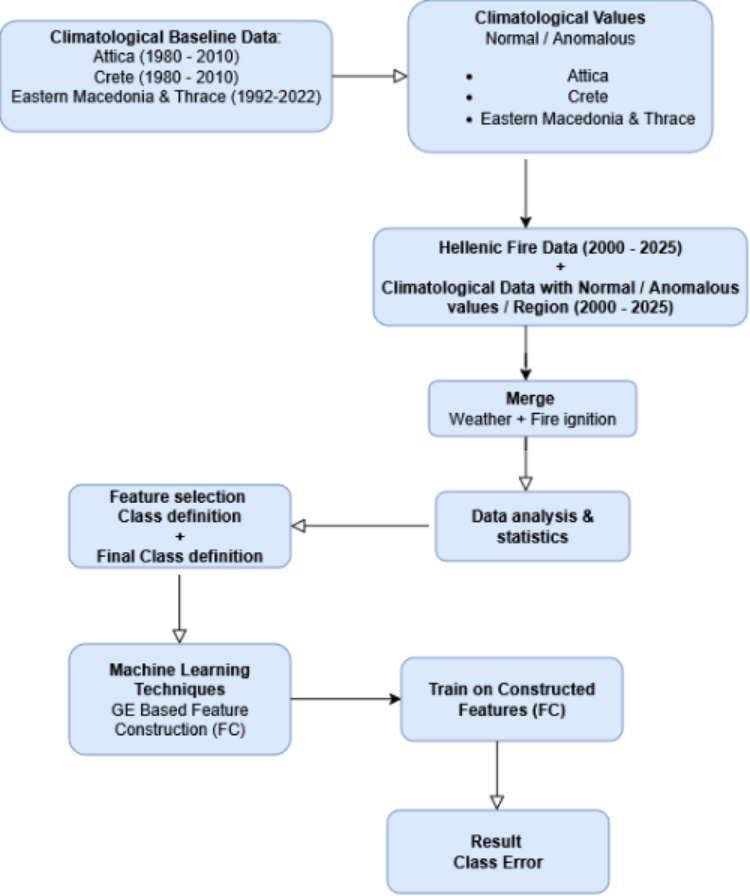
\includegraphics{process_FC}
\par\end{centering}
\end{figure}

Each experiment was executed 30 times, using different seeds for the
random number generator in every run. In addition, the ten fold cross
\nobreakdash- validation procedure was applied to ensure robust validation
of the experimental results. The proposed feature construction method
was applied independently to each fold, and the average classification
errors on the corresponding test sets were computed. 

To evaluate the predictive performance of the proposed feature construction
method against widely used machine learning approaches, five models
were trained and tested on the climatological and wildfire duration
records of the three study regions: a genetic-neuroevolution network
(NEAT) \citep{neat}, a radial basis function network (RBF) \citep{rbf1,rbf2},
a feedforward neural network trained with the Adam optimizer \citep{Adam,AdamNN},
a feedforward neural network trained with the L-BFGS algorithm \citep{lbfgs},
and the proposed feature construction method based on grammatical
evolution (FC2). Table \ref{tab:basic_tbl} reports the mean relative
error obtained by each method for Attica, Crete, and Eastern Macedonia
\& Thrace, together with the average performance across all three
regions.

\begin{table}[H]
\caption{Experimental results on the used datasets using a series of machine
learning methods.\label{tab:basic_tbl}}

\centering{}%
\begin{tabular}{|c|c|c|c|c|c|}
\hline 
DATASET & NEAT & RBF & ADAM & LBFGS & FC2\tabularnewline
\hline 
\hline 
ATTICA & 15.35\% & 4.81\% & 3.83\% & 2.98\% & 1.90\%\tabularnewline
\hline 
CRETE & 16.36\% & 1.79\% & 2.25\% & 3.70\% & 2.18\%\tabularnewline
\hline 
MACEDONIA & 14.24\% & 5.94\% & 7.56\% & 0.51\% & 0.46\%\tabularnewline
\hline 
AVERAGE & 15.32\% & 4.18\% & 4.55\% & 2.40\% & 1.51\%\tabularnewline
\hline 
\end{tabular}
\end{table}

The differences among the five methods, summarized numerically in
Table \ref{tab:basic_tbl}, are visualized in Figure \ref{fig:Graph}
to facilitate a direct region-by-region comparison. The chart highlights
that FC2 consistently ranks among the best-performing methods in Attica
and Eastern Macedonia \& Thrace, whereas in Crete the RBF network
marginally outperforms it. NEAT, in contrast, exhibits substantially
higher error across all three regions, underlining its limited suitability
for this prediction task.

\begin{figure}[H]
\begin{centering}
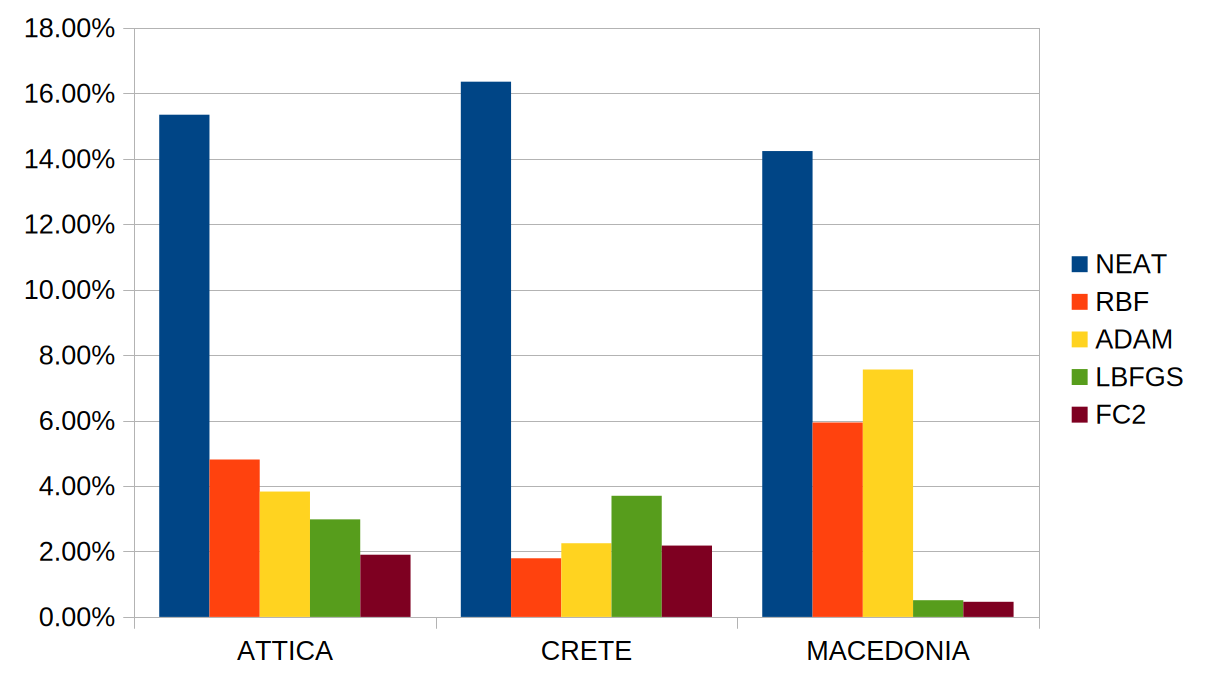
\includegraphics[scale=0.75]{allmethods}
\par\end{centering}
\caption{Graphical representation of the experimental results obtained by the
application of various machine learning methods.\label{fig:Graph}}

\end{figure}

Beyond the comparison against alternative methods, we further examined
how the number of features constructed by the grammatical evolution
process affects model accuracy. Figure \ref{fig:fcGraph} illustrates
the average error obtained when one, two, or three constructed features
($F=1,F=2,F=3$) are used as inputs. Across all three regions, the
error decreases as additional constructed features are introduced,
with the most pronounced improvement observed in Eastern Macedonia
\& Thrace, indicating that extracting more than a single derived feature
contributes measurably to the model's predictive capacity.

\begin{figure}[H]
\begin{centering}
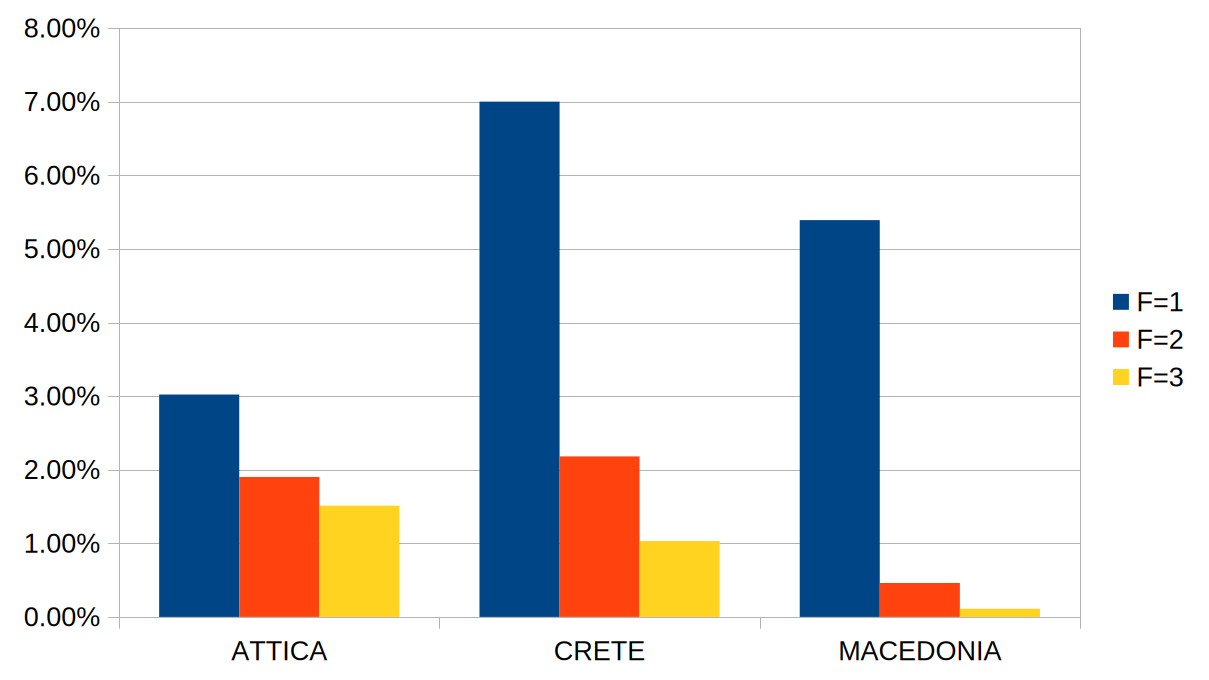
\includegraphics[scale=0.75]{fcmethods}
\par\end{centering}
\caption{Graphical representation of the average classification obtained by
the feature construction method using a variety of values for the
number of constructed features $\left(F=1,F=2,F=3\right)$.\label{fig:fcGraph}}

\end{figure}

The results of the statistical analysis are presented graphically
in Figure \ref{fig:stat_models}, where the mean error and standard
deviation of each method are shown alongside the corresponding significance
level relative to FC2. Although the Friedman test did not reach the
conventional 0.05 significance threshold (chi-squared = 8.533, $p=0.074$),
the Nemenyi critical difference of 3.522 confirms that the average
rank of FC2 differs significantly from that of NEAT, consistent with
the paired t-test result ($p=0.0002$). The remaining comparisons,
against LBFGS, RBF, and ADAM, do not reach statistical significance,
which is likely attributable to the small number of regions ($n=3$)
available for the paired tests.

\begin{figure}[H]
\begin{centering}
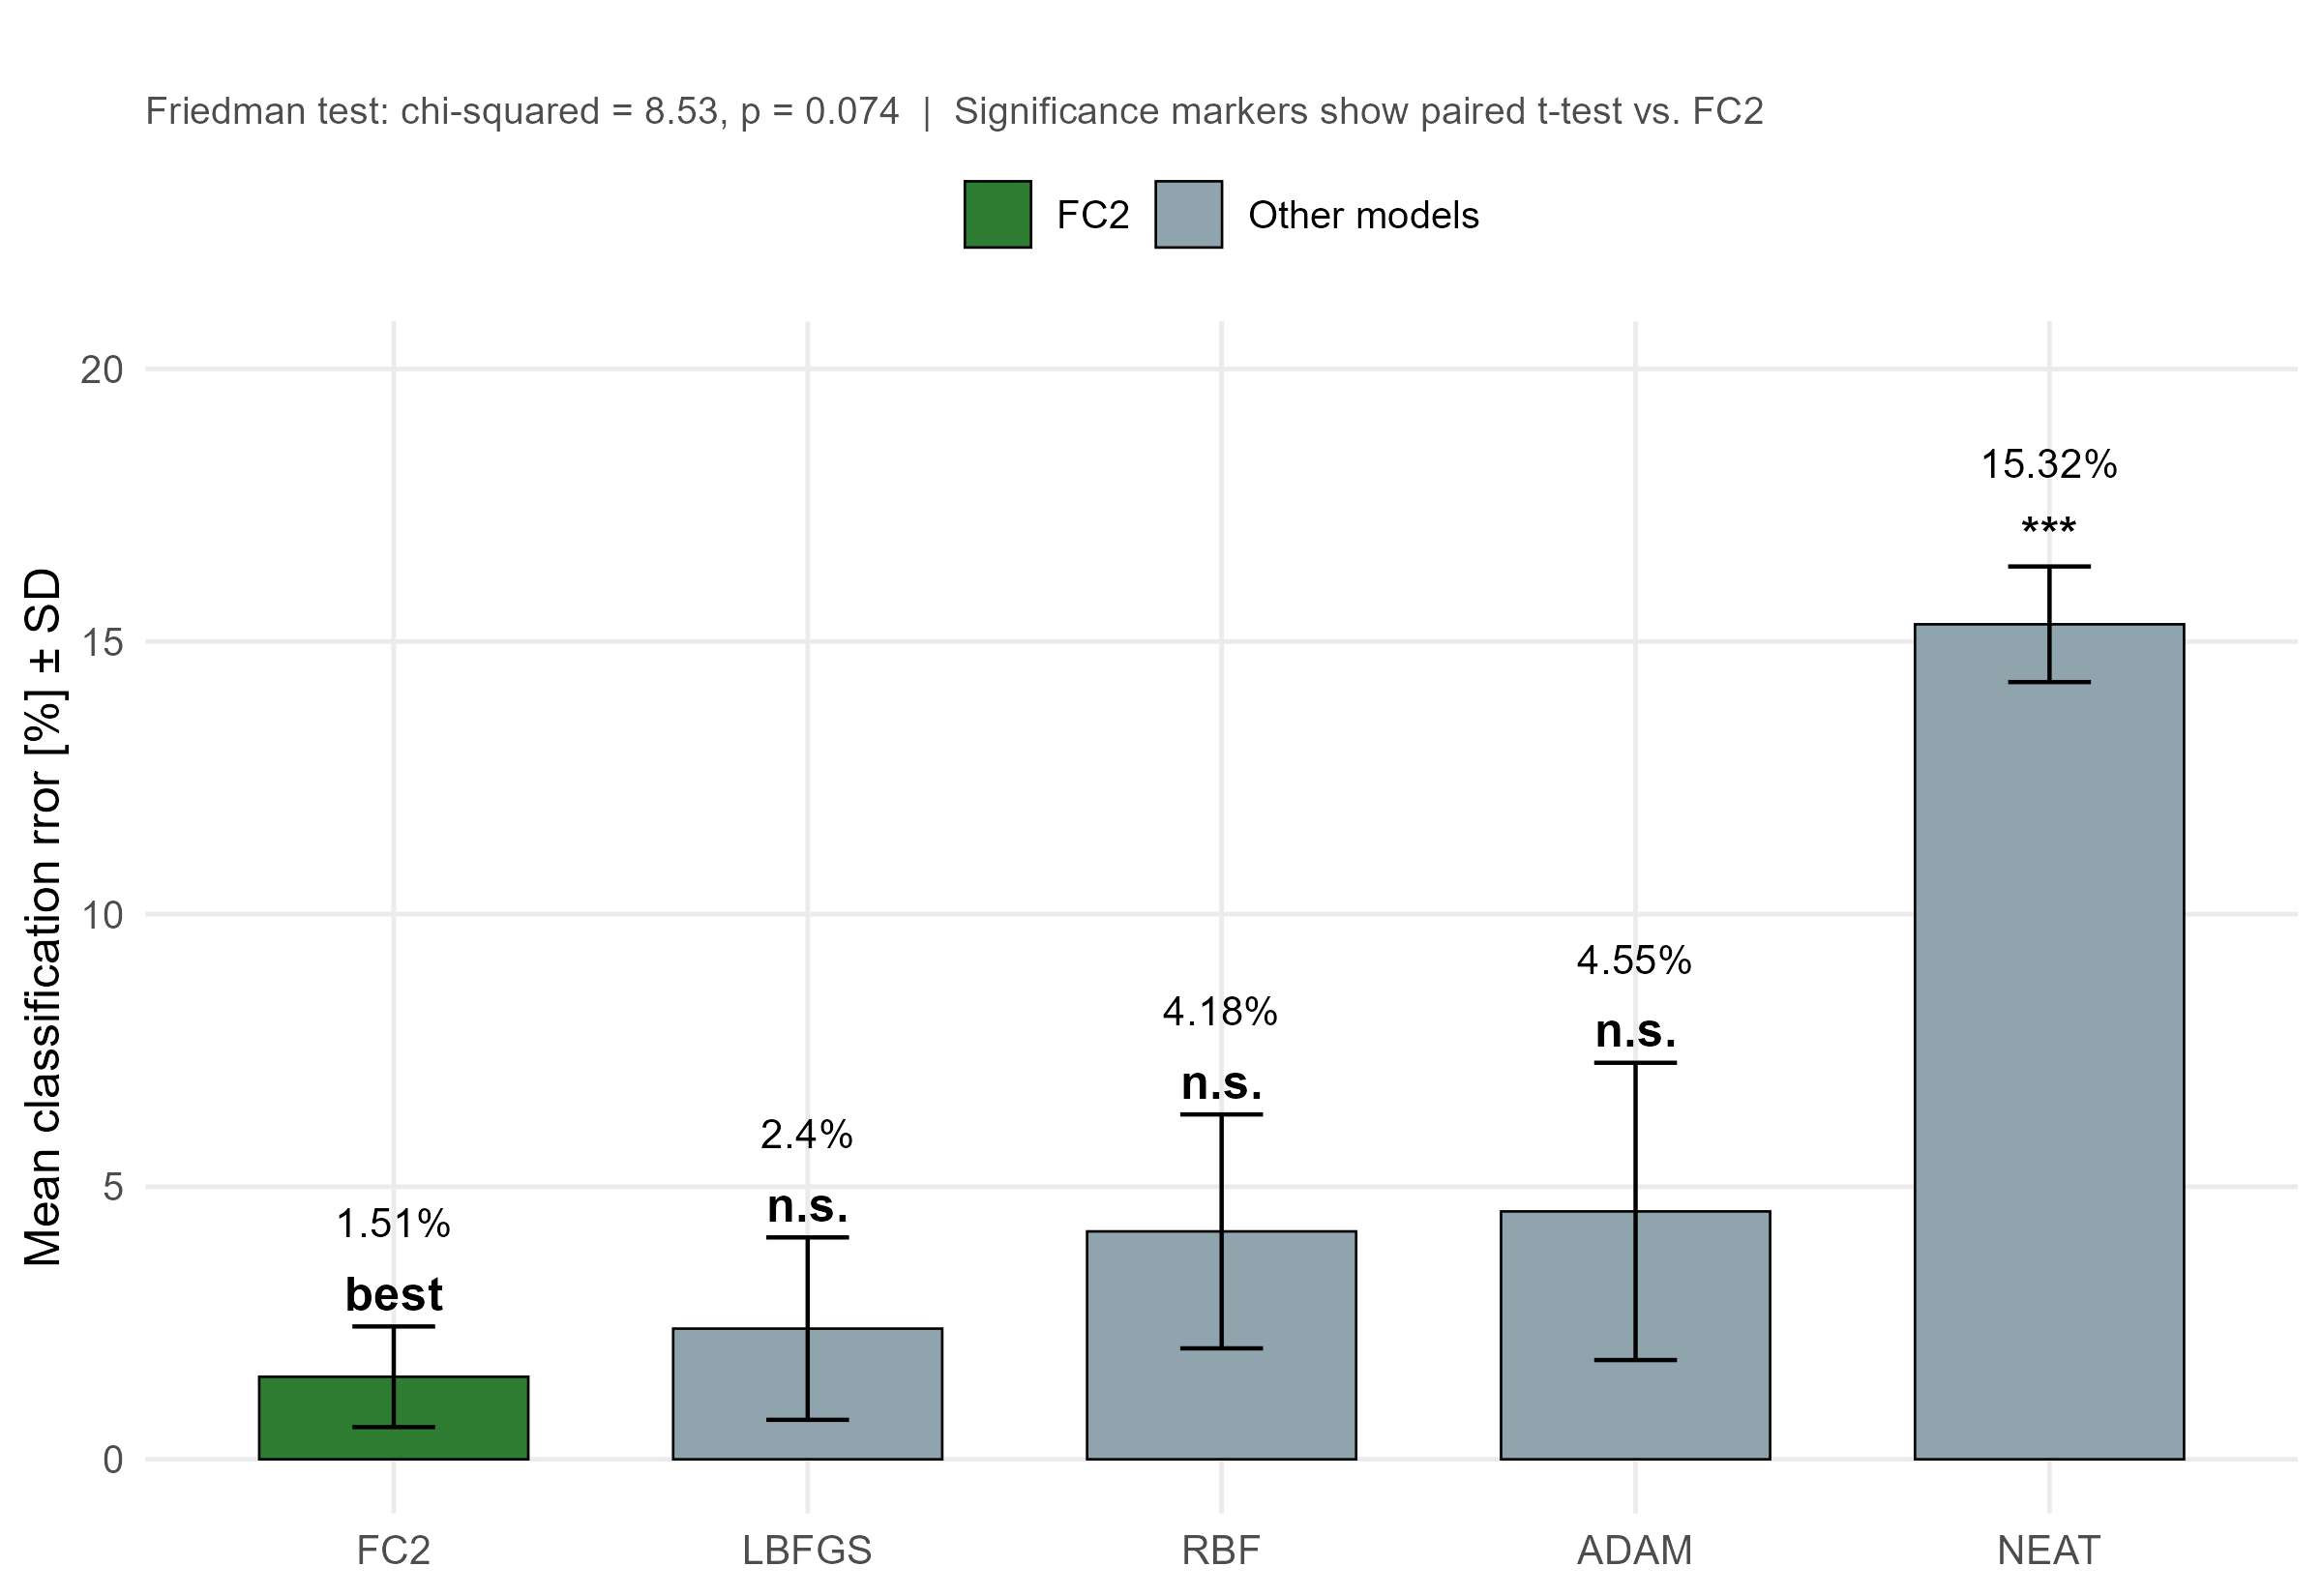
\includegraphics[scale=0.65]{statistical_analysis_figure}
\par\end{centering}
\caption{Mean prediction error per method with standard deviation and statistical
significance relative to FC2.\label{fig:stat_models}}
\end{figure}

To determine whether the observed differences in predictive accuracy
are statistically meaningful rather than attributable to chance, a
non-parametric Friedman test was applied across the three regions,
followed by pairwise comparisons of FC2 against each of the remaining
four methods using the paired Wilcoxon signed-rank test and the paired
t-test. Table \ref{tab:stattable} summarizes the descriptive statistics,
average ranks, and significance outcomes of these comparisons, using
FC2 as the reference method.

\begin{table}
\begin{centering}
\begin{tabular}{|c|c|c|c|c|c|c|c|c|c|}
\hline 
{\footnotesize\textbf{Model}} & \begin{cellvarwidth}[t]
\centering
{\footnotesize\textbf{Mean}}{\footnotesize\par}

{\footnotesize\textbf{Error}}
\end{cellvarwidth} & \begin{cellvarwidth}[t]
\centering
{\footnotesize\textbf{SD}}{\footnotesize\par}

{\footnotesize\textbf{Error}}
\end{cellvarwidth} & \begin{cellvarwidth}[t]
\centering
{\footnotesize\textbf{Min}}{\footnotesize\par}

{\footnotesize\textbf{Error}}
\end{cellvarwidth} & \begin{cellvarwidth}[t]
\centering
{\footnotesize\textbf{Max}}{\footnotesize\par}

{\footnotesize\textbf{Error}}
\end{cellvarwidth} & \begin{cellvarwidth}[t]
\centering
{\footnotesize\textbf{Avg}}{\footnotesize\par}

{\footnotesize\textbf{Rank}}
\end{cellvarwidth} & \begin{cellvarwidth}[t]
\centering
{\footnotesize\textbf{Mean Diff}}{\footnotesize\par}

{\footnotesize\textbf{vs FC2}}
\end{cellvarwidth} & {\footnotesize\textbf{Wilcoxon p}} & \begin{cellvarwidth}[t]
\centering
{\footnotesize\textbf{Paired}}{\footnotesize\par}

{\footnotesize\textbf{t\_p}}
\end{cellvarwidth} & {\footnotesize\textbf{Significance}}\tabularnewline
\hline 
\hline 
{\footnotesize FC2} & {\footnotesize 1.51} & {\footnotesize 0.92} & {\footnotesize 0.46} & {\footnotesize 2.18} & {\footnotesize 1.33} & {\footnotesize 0} &  &  & {\footnotesize Reference}\tabularnewline
\hline 
{\footnotesize LBFGS} & {\footnotesize 2.4} & {\footnotesize 1.67} & {\footnotesize 0.51} & {\footnotesize 3.7} & {\footnotesize 2.67} & {\footnotesize -0.88} & {\footnotesize 0.1814} & {\footnotesize 0.1798} & {\footnotesize n.s.}\tabularnewline
\hline 
{\footnotesize RBF} & {\footnotesize 4.18} & {\footnotesize 2.15} & {\footnotesize 1.79} & {\footnotesize 5.94} & {\footnotesize 2.67} & {\footnotesize -2.67} & {\footnotesize 0.4227} & {\footnotesize 0.2571} & {\footnotesize n.s.}\tabularnewline
\hline 
{\footnotesize ADAM} & {\footnotesize 4.55} & {\footnotesize 2.73} & {\footnotesize 2.25} & {\footnotesize 7.56} & {\footnotesize 3.33} & {\footnotesize -3.03} & {\footnotesize 0.1814} & {\footnotesize 0.286} & {\footnotesize n.s.}\tabularnewline
\hline 
{\footnotesize NEAT} & {\footnotesize 15.32} & {\footnotesize 1.06} & {\footnotesize 14.24} & {\footnotesize 16.36} & {\footnotesize 5} & {\footnotesize -13.8} & {\footnotesize 0.1814} & {\footnotesize 0.0002} & {\footnotesize{*}{*}{*}}\tabularnewline
\hline 
\end{tabular}
\par\end{centering}
\caption{Statistical comparison of the proposed FC2 method against NEAT, RBF,
ADAM, and LBFGS.\label{tab:stattable}}
\end{table}

{\footnotesize\textit{Friedman test: chi-squared = 8.533, df = 4,
p-value = 0.0739}}{\footnotesize\par}

{\footnotesize\textit{Nemenyi critical difference (alpha = 0.05):
3.522}}{\footnotesize\par}

{\footnotesize\textit{Significance vs. FC2 (paired t-test): {*}{*}{*}
p\textless 0.001, {*}{*} p\textless 0.01, {*} p\textless 0.05,
n.s. = not significant}}{\footnotesize\par}

\section{Conclusions\label{sec:Conclusions}}

This study developed and validated the climatological influences associated
with climate change for three climatically distinct regions of Greece,
namely Attica, Eastern Macedonia \& Thrace, and Crete, using forty
five years (1980--2025) of combined climatological and operational
fire incident data. Specifically, thirty years of climatological data
were used as the baseline, 1980--2010 for Attica and Crete, and 1992--2022
for Eastern Macedonia \& Thrace, due to the absence of earlier historical
records. Based on these data, classes were generated to define the
climatological normal values for each season, which were then compared
with the conditions observed during the 2000--2025 fire events. This
comparison allowed us to identify the anomalous climatological values
and assess their influence on the duration of each forest fire.

Finally, the Final\_effects class was generated from the combined
influence of temperature, humidity, and wind speed features, and its
reliability was validated using five machine learning techniques across
all three datasets. The machine learning techniques that validated
our results are: the NEAT method, the Radial Basis Function (RBF),
the LBFGS optimizer, the ADAM optimizer, and the Feature Construction
(FC2). The machine learning techniques successfully validated our
results, with the FC2 method based on Grammatical Evolution for constructing
new features, achieving the best overall performance with mean relative
error across all three regions at 1.51\%. Specifically, the error
rate for the Attica region was 1.90\% (98.10\% accuracy), for Crete
2.18\% (97.82\% accuracy), and for the Eastern Macedonia \& Thrace
region 0.46\% (99.54\% accuracy). It is worth noting that only for
the region of Crete did the RBF achieve a slightly better performance,
with an error rate of 1.79\%.

In addition, the statistical validation reinforces that the difference
between FC2 and NEAT is unlikely to be attributable to chance. The
overall Friedman test did not reach the conventional 0.05 significance
threshold (chi-squared = 8.533, p = 0.074), and the Nemenyi critical
difference of 3.522 confirms that the average rank of FC2 differs
significantly only from that of NEAT, while the differences from RBF,
LBFGS, and ADAM are not statistically significant. This outcome is
consistent with the paired t-test, which likewise shows a statistically
significant difference from NEAT (p = 0.0002), but not from the remaining
three methods.

\vspace{6pt}


\authorcontributions{Conceptualization, C.K. and I.G.T.; methodology, C.K.; software,
I.G.T.; validation, G.K. and V.C.; formal analysis, V.C.; investigation,
C.K.; resources, data curation, C.K.; writing---original draft preparation,
C.K.; writing---review and editing, I.G.T.; visualization, V.C.;
supervision, I.G.T.; project administration, I.G.T.; funding acquisition,
I.G.T. All authors have read and agreed to the published version of
the manuscript.}

\funding{This research has been financed by the European Union: Next Generation
EU through the Program Greece 2.0 National Recovery and Resilience
Plan, under the call RESEARCH---CREATE---INNOVATE, project name
“iCREW: Intelligent small craft simulator for advanced crew training
using Virtual Reality techniques” (project code:TAEDK-06195).}

\institutionalreview{Not applicable.}

\informedconsent{Not applicable.}

\dataavailability{The original contributions presented in this study are included in
the article. Further inquiries can be directed to the corresponding
author.}

\conflictsofinterest{The authors declare no conflicts of interest.}

\begin{adjustwidth}{-\extralength}{0cm}{}


\reftitle{References}
\begin{thebibliography}{999}
\bibitem{WMO}  WMO Climatological Normals. Available from: https://community.wmo.int/site/knowledge-hub/programmes-and-initiatives/climate-services/wmo-climatological-normals
(accessed on 16 July 2026).

\bibitem{Huntingford 2019}Huntingford, C., Jeffers, E. S., Bonsall,
M. B., Christensen, H. M., Lees, T., \& Yang, H. Machine learning
and artificial intelligence to aid climate change research and preparedness.
Environmental Research Letters, 2019. 14(12), 124007.

\bibitem{NASA 2023} NASA. Wildfires and Climate Change. Available
from: https://science.nasa.gov/earth/explore/wildfires-and-climate-change/
(accessed on 4 March 2026).

\bibitem{National Geographic}  National Geographic. Science. Available
from: https://www.nationalgeographic.com/science/article/climate-change-los-angeles-fire-wildfire
(accessed on 5 March 2026).

\bibitem{European Civil Protection} European Civil Protection and
Humanitarian Aid Operations. Wildfires. Available from: https://civil-protection-humanitarian-aid.ec.europa.eu/what/civil-protection/wildfires\_en
(accessed on 5 March 2026).

\bibitem{Flannigan et al.} Flannigan, M. D., \& Harrington, J. B.
(1988). A study of the relation of meteorological variables to monthly
provincial area burned by wildfire in Canada (1953--80). Journal
of Applied Meteorology (1988-2005), 441-452.

\bibitem{Swetnam 1993} Swetnam, T. W. (1993). Fire history and climate
change in giant sequoia groves. Science, 262(5135), 885-889.

\bibitem{Stocs et al.} Stocks, B. J., Fosberg, M. A., Lynham, T.
J., Mearns, L., Wotton, B. M., Yang, Q., ... \& McKenney, D. W. (1998).
Climate change and forest fire potential in Russian and Canadian boreal
forests. Climatic change, 38(1), 1-13.

\bibitem{Dale et al.} Dale, V. H., Joyce, L. A., McNulty, S., Neilson,
R. P., Ayres, M. P., Flannigan, M. D., ... \& Wotton, B. M. (2001).
Climate change and forest disturbances: climate change can affect
forests by altering the frequency, intensity, duration, and timing
of fire, drought, introduced species, insect and pathogen outbreaks,
hurricanes, windstorms, ice storms, or landslides. BioScience, 51(9),
723-734.

\bibitem{Flannigan 2000} Flannigan, M. D., Stocks, B. J., \& Wotton,
B. M. (2000). Climate change and forest fires. Science of the total
environment, 262(3), 221-229.

\bibitem{Flannigan 2006} Flannigan, M. D., Amiro, B. D., Logan, K.
A., Stocks, B. J., \& Wotton, B. M. (2006). Forest fires and climate
change in the 21st century. Mitigation and adaptation strategies for
global change, 11(4), 847-859.

\bibitem{Giannakopoulos 2011} Giannakopoulos, C., Kostopoulou, E.,
Varotsos, K. V., Tziotziou, K., \& Plitharas, A. An integrated assessment
of climate change impacts for Greece in the near future. Regional
Environmental Change, 2011. 11(4), 829-843.

\bibitem{Moritz et al.} Moritz, M. A., Parisien, M. A., Batllori,
E., Krawchuk, M. A., Van Dorn, J., Ganz, D. J., \& Hayhoe, K. (2012).
Climate change and disruptions to global fire activity. Ecosphere,
3(6), 1-22.

\bibitem{De Rigo}De Rigo, D., Libertà, G., Durrant, T. H., Vivancos,
T. A., \& San-Miguel-Ayanz, J. (2017). Forest fire danger extremes
in Europe under climate change: variability and uncertainty (Doctoral
dissertation, Publications Office of the European Union).

\bibitem{Di Virgilio 2019} Di Virgilio, G., Evans, J. P., Blake,
S. A., Armstrong, M., Dowdy, A. J., Sharples, J., \& McRae, R. (2019).
Climate change increases the potential for extreme wildfires. Geophysical
research letters, 46(14), 8517-8526.

\bibitem{Jones} Jones, M. W., Smith, A., Betts, R., Canadell, J.
G., Prentice, I. C., \& Le Quéré, C. (2020). Climate change increases
the risk of wildfires.

\bibitem{Jones 2022}Jones, M. W., Abatzoglou, J. T., Veraverbeke,
S., Andela, N., Lasslop, G., Forkel, M., ... \& Le Quéré, C. (2022).
Global and regional trends and drivers of fire under climate change.
Reviews of Geophysics, 60(3), e2020RG000726.

\bibitem{Jones 2024} Jones, M. W., Veraverbeke, S., Andela, N., Doerr,
S. H., Kolden, C., Mataveli, G., ... \& Abatzoglou, J. T. (2024).
Global rise in forest fire emissions linked to climate change in the
extratropics. Science, 386(6719), eadl5889.

\bibitem{Huang 2025} Huang, K., Wu, X., Zhang, L., Geng, H., \& Qu,
Y. (2025). Increasing risk of global forest loss from extreme wildfires
under climate change. International Journal of Digital Earth, 18(1),
2483982.

\bibitem{Forest Research} Forest Research.Climate change/Risks. Available
from: https://www.forestresearch.gov.uk/climate-change/risks/wildfire/
(accessed on 4 March 2026).

\bibitem{Optimus} Tsoulos, I. G., Charilogis, V., Kyrou, G., Stavrou,
V. N., \& Tzallas, A. (2025). OPTIMUS: A Multidimensional Global Optimization
Package. Journal of Open Source Software, 10(108), 7584.

\bibitem{Grammatical evolution 2001} O'Neill, M., \& Ryan, C. (2001).
Grammatical evolution. IEEE Transactions on Evolutionary Computation,
5(4), 349-358.

\bibitem{FC construct} Tsoulos, I., Gavrilis, D., \& Glavas, E. (2008).
Neural network construction and training using grammatical evolution.
Neurocomputing, 72(1-3), 269-277.

\bibitem{QFC} Tsoulos, I. G. (2022). QFC: A Parallel Software Tool
for Feature Construction, Based on Grammatical Evolution. Algorithms,
15(8), 295.

\bibitem{Weka 2016} Frank, E., Hall, M. A., \& Witten, I. H. (2016).
The WEKA Workbench. Online Appendix for\textquotedbl{} Data Mining:
Practical Machine Learning Tools and Techniques\textquotedbl .

\bibitem{Tsoulos 2022} Tsoulos, I. G. (2022). Constructing Features
Using a Hybrid Genetic Algorithm. Signals, 3(2), 174-188.

\bibitem{Tsoulos covid} Tsoulos, I. G., Tzallas, A. T., \& Tsalikakis,
D. (2022). Prediction of covid-19 cases using constructed features
by grammatical evolution. Symmetry, 14(10), 2149. 

\bibitem{Tsoulos fires} Kopitsa, C., Tsoulos, I. G., Miltiadous,
A., \& Charilogis, V. (2025). Predicting the Forest Fire Duration
Enriched with Meteorological Data Using Feature Construction Techniques.
Symmetry, 17(11), 1785.

\bibitem{Tsoulos parkinson} Psathas, A., Tsoulos, I. G., Giannakeas,
N., Tzallas, A., \& Charilogis, V. (2025). Constructing Artificial
Features with Grammatical Evolution for the Motor Symptoms of Parkinson’s
Disease. Bioengineering, 12(12), 1318.

\bibitem{Lillywhite object} Lillywhite, K., Lee, D. J., Tippetts,
B., \& Archibald, J. (2013). A feature construction method for general
object recognition. Pattern Recognition, 46(12), 3300-3314.

\bibitem{Lensen image} Lensen, A., Al-Sahaf, H., Zhang, M., \& Xue,
B. (2016, March). Genetic programming for region detection, feature
extraction, feature construction and classification in image data.
In European conference on genetic programming (pp. 51-67). Cham: Springer
International Publishing.

\bibitem[(2025)]{neat}K. O. Stanley, R. Miikkulainen, Evolving Neural
Networks through Augmenting Topologies, Evolutionary Computation \textbf{10},
pp. 99-127, 2002.

\bibitem[(1991)]{rbf1}J. Park and I. W. Sandberg, Universal Approximation
Using Radial-Basis-Function Networks, Neural Computation \textbf{3},
pp. 246-257, 1991.

\bibitem{rbf2}G.A. Montazer, D. Giveki, M. Karami, H. Rastegar, Radial
basis function neural networks: A review. Comput. Rev. J \textbf{1},
pp. 52-74, 2018.

\bibitem{Adam}D. P. Kingma, J. L. Ba, ADAM: a method for stochastic
optimization, in: Proceedings of the 3rd International Conference
on Learning Representations (ICLR 2015), pp. 1--15, 2015.

\bibitem{AdamNN}Y. Xue, Y. Tong, F. Neri, An ensemble of differential
evolution and Adam for training feed-forward neural networks. Information
Sciences \textbf{608}, pp. 453-471, 2022.

\bibitem{lbfgs}Liu, D. C., \& Nocedal, J. (1989). On the limited
memory BFGS method for large scale optimization. Mathematical programming,
45(1), 503-528.

\end{thebibliography}
%%%%%%%%%%%%%%%%%%%%%%%%%%%%%%%%%%%%%%%%%%
%% for journal Sci
%\reviewreports{\\
%Reviewer 1 comments and authors' response\\
%Reviewer 2 comments and authors' response\\
%Reviewer 3 comments and authors' response
%}
%%%%%%%%%%%%%%%%%%%%%%%%%%%%%%%%%%%%%%%%%%

\PublishersNote{}

\end{adjustwidth}{}
\end{document}
